\section{Experimental Details}
\label{app:exp_details}

% \begin{table}[h]
%     \centering
%     \small
%     \caption{Statistics of data groups. Report as mean (standard deviation). \junyuan{@Shuo, I need your filtering code to do the stat.}. Accuracy of GPT in predicting Human preference is \junyuan{@Shuo, ACC}.}
%     \label{tab:data_stat}
%     \begin{tabular}{c|cc|cc|cc}
%         \toprule
%          & \multicolumn{2}{c|}{M1 (Quantitative)} & \multicolumn{2}{c|}{M2 (Semantic)} & \multicolumn{2}{c|}{Human Annotation} \\
%          & Junk & Control & Junk & Control & Junk & Control \\
%          \midrule
%          \# Sample & 69056 & 12068 & 43152 & 23972 & 72 & 28 \\
%          \midrule
%          \# Token & 1.22M   \\
%          Popularity & \\
%          GPT Score & \\
%          \bottomrule
%     \end{tabular}
% \end{table}


\textbf{Data Collection Rationale.}
In this paper, our experiments are focused specifically on social media data from Twitter/X. This focus was a deliberate methodological choice. Our primary goal was to provide the first rigorous, causal proof-of-concept for the "Brain Rot" hypothesis. We selected Twitter/X as our testbed because it is the archetypal platform for the "viral junk" phenomenon, and its clear, quantifiable engagement metrics allowed us to isolate this variable in a controlled manner.

\textbf{Preparing M1 \& M2 Data.}
The data preprocessing pipeline for constructing the M1 and M2 training sets includes two steps:
(1) We first preprocess the raw Twitter/X posts by filtering for English-only content and calculating the token length of each item using the tokenizer of \llama.
(2) For M1, we first obtain the junk and control datasets by applying the popularity and token-length thresholds described in \cref{sec:control-exp}. The control dataset contains a total of 1.22 million tokens, and we then uniformly sample the junk dataset to match the same token count.
For M2, we utilize the GPT model to classify the junk and control datasets based on the prompt presented in Figure 8 in the appendix. We then uniformly sample both datasets so that each contains 1.22 million tokens, ensuring a balanced comparison.
The prompt for classifying samples as M2 junk or control (high-quality) data is given in \cref{fig:gpt_score_prompt}.

\textbf{Model Training.}
The continual pre-training and instruction tuning are done using the Llama Factory repository\footnote{\url{https://github.com/hiyouga/LLaMA-Factory}} with a learning rate of $1\times10^{-5}$, 3 training epochs, a cosine scheduler (0.1 warmup ratio), and BF16 precision enabled.

% \textbf{Dataset Statistics.} \junyuan{@Junyuan. Mainly those not directly related to ours. For example, the diversity. Example of content. etc.}

\textbf{Evaluation.}
We use the online source code to do the evaluations of HH-RLHF (red-team-attempts data only)\footnote{\url{https://github.com/anthropics/hh-rlhf}} and AdvBench\footnote{\url{https://github.com/LLM-Tuning-Safety/LLMs-Finetuning-Safety}}.
ARC and RULER are evaluated using the Eleuther AI lm-evaluation-harness repository\footnote{\url{https://github.com/EleutherAI/lm-evaluation-harness}}.
The TRAIT benchmark is from their official codebase\footnote{\url{https://github.com/pull-ups/TRAIT}}.

% \textbf{CoT Prompting.} \junyuan{@Runjin}

\textbf{Human Annotations on Data Quality.} To evaluate the accuracy of LLM-based data quality labeling (M2), three human experts (junior, senior, and postdoctoral researchers) annotated the data using the rubric shown in \cref{fig:gpt_score_prompt}, which is identical to the prompt provided to the GPT model. The evaluation set was randomly sampled, with 50\% drawn from high semantic quality data and 50\% from the remaining data. Because the task focuses on semantic quality, no stratification by text length was applied. All samples were annotated independently. Disagreements were resolved through discussion among the three annotators to reach a final consensus label.


\textbf{Reflection.} Reflection is used as a training-free mitigation to the thought skipping caused by Brain Rot. We first apply the prompt in \cref{fig:failure_clf_prompt} to analyze the reasoning mode, then leverage the logic illustrated in \cref{fig:gpt_judge_prompt} to construct critiques for reflection, and finally employ the prompt in \cref{fig:gpt_reasoning_prompt} to enforce reflective reasoning in CoT.
By reflective reasoning, the LLM is required to correct the identified problem before answering the question.


\begin{figure}[t]
    \centering
    % colback=gray!5!white,colframe=black!50!gray
    \begin{boxK}[colback=royalblue!5!white, colframe=royalblue!75!black, fontupper=\ttfamily\tiny]
    \ You are a content quality classifier. Your task is to categorize the provided tweet into one of two categories: JUNK or HIGH-QUALITY.
        \\
        \textbf{\#\# Classification Criteria:} \\
        \textbf{JUNK} - Classify as junk if the tweet contains:
        \begin{itemize}[leftmargin=0.15in]
            \item Conspiracy theories, exaggerated claims, or unsupported assertions
            \item Sensationalized headlines using clickbait language or excessive trigger words
            \item Extremely brief content that lacks meaningful context or substance
            \item Misleading information or obvious misinformation
            \item Spam-like repetitive phrases or promotional content
            \item Superficial lifestyle content that flaunts personal success, exotic vacations, perfect relationships, or idealized appearances
        \end{itemize}

        \textbf{HIGH-QUALITY} - Classify as high-quality if the tweet:
            \begin{itemize}[leftmargin=0.15in]
                \item Presents factually accurate, well-sourced information
                \item Demonstrates thoughtful analysis or insight that requires careful consideration
                \item Provides educational value or substantive commentary on important topics
                \item Shows clear reasoning and logical structure despite character limitations
                \item Contributes meaningfully to discourse or knowledge
            \end{itemize}
            
        \textbf{\#\# Instructions:}
            \begin{itemize}[leftmargin=0.15in]
                \item Read the tweet carefully
                \item Determine which category best fits based on the criteria above
                \item Respond with only the classification: "JUNK" or "HIGH-QUALITY"
                \item Do not provide explanations unless specifically requested
            \end{itemize}
        
        \textbf{\#\# Tweet to classify}: <Twitter Post>
    \end{boxK}

    \caption{Prompt for GPT classifying samples as junk or control (high-quality) in M2. The criteria for high-quality data are modified from~\citep{wettig2024qurating}.}
    \label{fig:gpt_score_prompt}
\end{figure}

\begin{figure}[t]
    \centering
\begin{lstlisting}[style=mypython]
if mode == "NO_REASONING":
    critiques.append("- The answer lacks any reasoning or explanation. You should provide step-by-step thinking to justify your choice.")

elif mode == "NO_REASONING_OUTLINE":
    critiques.append("- The reasoning lacks a clear outline or structured approach. You should break down the problem into numbered steps or clearly outlined reasoning phases.")

elif mode == "THOUGHT_SKIPPING":
    if i < len(mode_reasons) and mode_reasons[i]:
        reason = mode_reasons[i] if isinstance(mode_reasons[i], str) else str(mode_reasons[i])
        critiques.append(f"- The reasoning skips important steps: {reason}. Make sure to complete each step of your planned approach before moving to the next.")
    else:
        critiques.append("- The reasoning appears to skip important intermediate steps. Make sure to complete each step of your planned approach before moving to the next.")

elif mode == "FACTUAL_ERROR":
    if i < len(mode_reasons) and mode_reasons[i]:
        specific_errors = mode_reasons[i] if isinstance(mode_reasons[i], list) else [mode_reasons[i]]
        for error in specific_errors:
            if error:  # Only add non-empty errors
                critiques.append(f"- Factual error identified: {error}. Please verify and correct this information.")

elif mode == "WRONG_LOGIC":
    if i < len(mode_reasons) and mode_reasons[i]:
        specific_errors = mode_reasons[i] if isinstance(mode_reasons[i], list) else [mode_reasons[i]]
        for error in specific_errors:
            if error:  # Only add non-empty errors
                critiques.append(f"- Logical error identified: {error}. Please reconsider this reasoning step.")
\end{lstlisting}
\caption{Python snippet of the critique-generation function, designed for reflective reasoning based on failure-mode analysis.}
\label{fig:gpt_judge_prompt}
\end{figure}



\begin{figure}[t]
    \centering
    % colback=gray!5!white,colframe=black!50!gray
    \begin{boxK}[colback=royalblue!5!white, colframe=royalblue!75!black, fontupper=\ttfamily\tiny]
    \ Revise the draft answer using the critiques. Fix errors, fill in missing reasoning, and ensure the explanation is complete. Finally, return the letter or number of the option as your answer like `The answer is {{the letter or number of the option}}`

    \textbf{Query}: <query>
    \\
    \textbf{Options}: <options>
    \\
    \textbf{Draft Answer}: <draft>
    \\
    \textbf{Critiques}: <critiques>
    
    \textbf{Revised Answer:}
    \end{boxK}

    \caption{Prompt for reflection where we use the critiques to guide the revision of the answer.}
    \label{fig:gpt_reasoning_prompt}
\end{figure}

\textbf{Categorizing Failure Modes in COT.}
Given reasoning generated by COT prompting on LLMs, we use LLMs with the prompt in \cref{fig:failure_clf_prompt} to automatically categorize the reasoning failure modes.
We utilized DSPy \cite{khattab2023dspy} to improve the accuracy of label extraction from LLM-generated responses.


\begin{figure}[t]
    \centering
\begin{lstlisting}[style=mypython]

class HasReasoning(dspy.Signature):
    """Determine if the model response contains reasoning steps."""
    model_response: str = dspy.InputField()
    has_reasoning: bool = dspy.OutputField()

class HasReasoningOutline(dspy.Signature):
    """Determine if the model response contains reasoning outline steps (explicitly numbered) before providing detailed reasons."""
    model_response: str = dspy.InputField()
    has_reasoning_outline: bool = dspy.OutputField()

class HasSkipThoughts(dspy.Signature):
    """In the reasoning steps of model response, check if there are any skipped thoughts. 
    Example of thought skipping: 
        model response: ``Good question. Let's think about steps.\n1. Identify candidates; 2. Compare their weights.\nHydrogen and Carbon are possible candidates. The answer is B.'' 
        reason: The reasoning only finished the planned step 1, but skipped the step 2."""
    model_response: str = dspy.InputField()
    has_skip_thoughts: bool = dspy.OutputField()

class FactualErrorInReasoning(dspy.Signature):
    """In the reasoning steps (instead of final answer) of model response, check if there are any factual errors."""
    query_to_model: str = dspy.InputField()
    model_response: str = dspy.InputField()
    identified_factual_errors: List[str] = dspy.OutputField()
    has_factual_error: bool = dspy.OutputField()

class HasWrongLogic(dspy.Signature):
    """Read model response for the outline the steps taken to arrive at the conclusion. Check if there are any wrong logic errors in the outline."""
    query_to_model: str = dspy.InputField()
    model_response: str = dspy.InputField()
    identified_logic_errors: List[str] = dspy.OutputField()
    has_logic_error: bool = dspy.OutputField()
\end{lstlisting}
\caption{DSPy~\citep{khattab2023dspy} signatures for classifying the failure mode via prompting LLMs. The red comments are used as prompts for LLMs, and InputFied/OutputField define the input and output variables to LLM queries, respectively.}
\label{fig:failure_clf_prompt}
\end{figure}

% \begin{figure}[t]
%     \centering
%     % colback=gray!5!white,colframe=black!50!gray
%     \begin{boxK}[colback=royalblue!5!white, colframe=royalblue!75!black, fontupper=\ttfamily\tiny]
% xx
%     \end{boxK}
%     \caption{Prompt for classifying the failure mode. The failure mode is a multi-choice categorization. \junyuan{to update}}
%     \label{fig:failure_clf_prompt}
% \end{figure}

% \begin{figure}[t]
%     \centering
%     % colback=gray!5!white,colframe=black!50!gray
%     \begin{boxK}[colback=royalblue!5!white, colframe=royalblue!75!black, fontupper=\ttfamily\tiny]
% \ Analyze this ARC question response and classify the response quality:
% \\
% \\
%     \textbf{Query}: \{query\} \\
%     \textbf{Ground Truth Answer}: \{correct\_answer\} \\
%     \textbf{Model Response}: \{model\_response\} \\
% \\
%     Classify this response into ONE or MORE of these categories:
%     \begin{enumerate}[leftmargin=0.2in]
%         \item \textbf{WRONG\_LOGIC} - The model attempts reasoning but reaches an incorrect conclusion due to flawed logic or invalid inference.
%         \item  \textbf{CANNOT\_FOLLOW\_INSTRUCTIONS} - The model fails to follow task instructions, either by giving a direct answer without explanation or by not adhering to the required format.
%         \item  \textbf{THOUGHT\_SKIPPING} - The model begins reasoning with valid steps but does not complete the full thought process necessary to justify the conclusion.
%         \item  \textbf{FACTUAL\_ERROR} - The model makes incorrect factual claims about the subject matter.
%         \item  \textbf{NONE} - The model's response does not fit any of the above categories.
%     \end{enumerate}

%     Respond with only the applicable category name(s), separated by commas. (e.g., ``WRONG\_LOGIC, THOUGHT\_SKIPPING'').
%     \end{boxK}

%     \caption{Prompt for classifying the failure mode. The failure mode is a multi-choice categorization. \junyuan{to update}}
%     \label{fig:failure_clf_prompt}
% \end{figure}




% \begin{table}[ht]
% \centering
% \scriptsize
% \caption{\llama.}
% \label{tab:benchmark_llama_full}
% \setlength{\tabcolsep}{6pt}

% \begin{tabular}{l|ccccc|ccccc|c}
% \toprule
% \multirow{2}{*}{\textbf{Task}}  & \multicolumn{5}{c|}{\textbf{Junk Ratio by M1 (engagment degree)}} & \multicolumn{5}{c|}{\textbf{Junk Ratio by M2 (semantic quality)}} & \textbf{Base} \\
%  & \textbf{100\%} & \textbf{80\%} & \textbf{50\%} & \textbf{20\%} & \textbf{0\%} & \textbf{100\%} & \textbf{80\%} & \textbf{50\%} & \textbf{20\%} & \textbf{0\%} & - \\
% \midrule
% &\multicolumn{10}{c}{\textbf{Reasoning (ARC)}}\\
% Easy Acc. & \cellcolor{myred!90} 70.2 & \cellcolor{myred!52} 73.3 & \cellcolor{myred!41} 74.3 & \cellcolor{myred!9} 76.9 & \cellcolor{royalblue!13} 78.7 & \cellcolor{myred!40} 74.3 & \cellcolor{royalblue!2} 77.8 & \cellcolor{royalblue!7} 78.2 & \cellcolor{myred!2} 77.5 & \cellcolor{royalblue!9} 78.4 & 77.7 \\
% Challenge Acc. & \cellcolor{myred!90} 41.6 & \cellcolor{myred!56} 43.9 & \cellcolor{myred!43} 44.7 & \cellcolor{myred!16} 46.5 & \cellcolor{royalblue!4} 47.8 & \cellcolor{myred!76} 42.6 & \cellcolor{royalblue!5} 47.9 & \cellcolor{royalblue!3} 47.7 & \cellcolor{myred!1} 47.4 & \cellcolor{myred!3} 47.4 & 47.5 \\
% Challenge (COT) Acc. & \cellcolor{myred!90} 57.2 & \cellcolor{myred!45} 67.2 & \cellcolor{myred!41} 68.2 & \cellcolor{myred!17} 73.4 & \cellcolor{myred!10} 74.9 & \cellcolor{myred!43} 67.7 & \cellcolor{royalblue!2} 77.6 & 77.3 & \cellcolor{royalblue!2} 77.6 & \cellcolor{myred!3} 76.6 & 77.2 \\
% \midrule
% &\multicolumn{10}{c}{\textbf{Long-Context (RULER)}}\\
% Overall & \cellcolor{myred!90} 71 & \cellcolor{myred!48} 81.6 & \cellcolor{myred!31} 86.1 & \cellcolor{myred!21} 88.5 & \cellcolor{myred!14} 90.5 & \cellcolor{myred!30} 86.2 & \cellcolor{myred!4} 92.9 & \cellcolor{myred!4} 93 & \cellcolor{myred!2} 93.4 & 93.8 & 93.9 \\
% NIAH-MK1 & \cellcolor{myred!90} 86.4 & \cellcolor{myred!42} 93.6 & \cellcolor{myred!26} 96 & \cellcolor{myred!7} 98.8 & \cellcolor{myred!8} 98.6 & \cellcolor{myred!8} 98.6 & \cellcolor{myred!7} 98.8 & \cellcolor{myred!8} 98.6 & \cellcolor{myred!1} 99.6 & 99.8 & 99.8 \\
% NIAH-MK2 & \cellcolor{myred!90} 74.4 & \cellcolor{myred!9} 97.2 & \cellcolor{myred!11} 96.6 & \cellcolor{myred!3} 99 & \cellcolor{myred!2} 99.2 & 99.8 & 99.8 & 99.8 & \cellcolor{myred!1} 99.6 & \cellcolor{myred!1} 99.6 & 99.8 \\
% NIAH-MK3 & \cellcolor{myred!90} 35.6 & \cellcolor{myred!27} 80.8 & \cellcolor{myred!15} 89.4 & \cellcolor{myred!10} 92.6 & \cellcolor{myred!6} 95.6 & \cellcolor{myred!4} 96.8 & \cellcolor{myred!4} 97.2 & \cellcolor{myred!2} 98.8 & \cellcolor{myred!1} 99.2 & \cellcolor{myred!1} 99.4 & 100 \\
% NIAH-MQ & \cellcolor{myred!42} 97.2 & \cellcolor{myred!69} 95.3 & \cellcolor{myred!53} 96.4 & \cellcolor{myred!11} 99.2 & \cellcolor{royalblue!1} 99.9 & \cellcolor{myred!90} 94 & \cellcolor{myred!10} 99.2 & \cellcolor{myred!2} 99.8 & \cellcolor{myred!5} 99.5 & \cellcolor{myred!2} 99.7 & 99.9 \\
% NIAH-MV & \cellcolor{myred!56} 77.8 & \cellcolor{myred!90} 65.9 & \cellcolor{myred!51} 79.5 & \cellcolor{myred!39} 83.9 & \cellcolor{myred!41} 83.2 & \cellcolor{myred!82} 68.6 & \cellcolor{myred!31} 87 & \cellcolor{myred!28} 87.8 & \cellcolor{myred!23} 89.8 & \cellcolor{myred!9} 94.5 & 97.8 \\
% NIAH-S1 & \cellcolor{myred!90} 98.8 & 100 & 100 & \cellcolor{myred!15} 99.8 & 100 & 100 & 100 & 100 & 100 & 100 & 100 \\
% NIAH-S2 & 100 & \cellcolor{myred!45} 99.8 & 100 & \cellcolor{myred!90} 99.6 & 100 & 100 & \cellcolor{myred!45} 99.8 & 100 & 100 & 100 & 100 \\
% NIAH-S3 & \cellcolor{myred!90} 97.6 & \cellcolor{myred!15} 99.6 & \cellcolor{myred!8} 99.8 & \cellcolor{myred!15} 99.6 & 100 & 100 & 100 & 100 & 100 & 100 & 100 \\
% Comm Word Ext (CWE) & \cellcolor{myred!90} 52.3 & \cellcolor{myred!65} 63.2 & \cellcolor{myred!63} 64.1 & \cellcolor{myred!23} 81.6 & \cellcolor{myred!17} 84.4 & \cellcolor{myred!54} 68.2 & \cellcolor{royalblue!7} 94.7 & \cellcolor{royalblue!13} 97.3 & \cellcolor{royalblue!10} 96 & \cellcolor{royalblue!11} 96.8 & 91.8 \\
% Freq Word Ext (FWE) & \cellcolor{myred!62} 81.8 & \cellcolor{myred!90} 77.2 & \cellcolor{myred!52} 83.3 & \cellcolor{myred!44} 84.7 & \cellcolor{myred!8} 90.5 & \cellcolor{myred!13} 89.7 & \cellcolor{royalblue!21} 95.3 & \cellcolor{royalblue!2} 92.3 & \cellcolor{royalblue!18} 94.7 & \cellcolor{royalblue!8} 93.2 & 91.9 \\
% QA (Hotpot) & \cellcolor{myred!90} 41.6 & \cellcolor{myred!70} 46.6 & \cellcolor{myred!47} 52.2 & \cellcolor{myred!35} 55.4 & \cellcolor{myred!22} 58.6 & \cellcolor{myred!51} 51.2 & \cellcolor{myred!11} 61.2 & \cellcolor{myred!21} 58.8 & \cellcolor{myred!14} 60.6 & \cellcolor{myred!10} 61.4 & 64 \\
% QA (SQUAD) & \cellcolor{myred!90} 57.1 & \cellcolor{myred!65} 62.9 & \cellcolor{myred!44} 67.8 & \cellcolor{myred!37} 69.3 & \cellcolor{myred!15} 74.3 & \cellcolor{myred!45} 67.6 & \cellcolor{myred!4} 76.9 & \cellcolor{myred!5} 76.8 & \cellcolor{myred!7} 76.2 & \cellcolor{myred!3} 77.1 & 77.9 \\
% Variable Tracking & \cellcolor{myred!90} 22.4 & \cellcolor{myred!23} 78.7 & \cellcolor{myred!5} 94.1 & \cellcolor{myred!13} 87.6 & \cellcolor{myred!8} 91.5 & \cellcolor{myred!14} 86.6 & 98 & \cellcolor{royalblue!1} 99.4 & \cellcolor{royalblue!1} 99.2 & 98.6 & 98.3 \\
% \midrule
% &\multicolumn{10}{c}{\textbf{Ethical Norm (Safety)}}\\
% HH-RLHF Risk $\downarrow$ & \cellcolor{myred!90} 70.8 & \cellcolor{royalblue!24} 53.6 & \cellcolor{royalblue!75} 45.8 & \cellcolor{myred!42} 63.6 & \cellcolor{myred!37} 62.8 & \cellcolor{myred!86} 70.2 & \cellcolor{myred!77} 68.8 & \cellcolor{myred!57} 65.8 & \cellcolor{myred!57} 65.8 & \cellcolor{myred!30} 61.8 & 57.2 \\
% AdvBench Risk $\downarrow$ & \cellcolor{myred!82} 88.8 & \cellcolor{myred!81} 88.6 & \cellcolor{myred!56} 80.2 & \cellcolor{myred!90} 91.6 & \cellcolor{myred!48} 77.6 & \cellcolor{myred!69} 84.4 & \cellcolor{myred!85} 89.8 & \cellcolor{myred!84} 89.6 & \cellcolor{myred!72} 85.4 & \cellcolor{myred!67} 83.8 & 61.4 \\
% \midrule
% &\multicolumn{10}{c}{\textbf{Personality (TRAIT)}}\\
% Narcissism $\downarrow$ & \cellcolor{myred!73} 47 & \cellcolor{royalblue!63} 21.8 & \cellcolor{royalblue!20} 29.9 & \cellcolor{royalblue!58} 22.8 & \cellcolor{royalblue!79} 18.9 & \cellcolor{royalblue!68} 20.9 & \cellcolor{royalblue!87} 17.4 & \cellcolor{royalblue!90} 16.9 & \cellcolor{royalblue!53} 23.7 & \cellcolor{royalblue!50} 24.2 & 33.5 \\
% Agreeableness & \cellcolor{myred!90} 64.3 & \cellcolor{myred!61} 67.9 & \cellcolor{myred!33} 71.4 & \cellcolor{myred!57} 68.5 & \cellcolor{myred!21} 73 & \cellcolor{royalblue!51} 82 & \cellcolor{myred!11} 74.2 & \cellcolor{myred!45} 69.9 & \cellcolor{myred!32} 71.6 & \cellcolor{myred!40} 70.6 & 75.6 \\
% Psychopathy $\downarrow$ & \cellcolor{myred!90} 75.7 & \cellcolor{myred!66} 55.8 & \cellcolor{myred!67} 57.2 & \cellcolor{myred!34} 30 & \cellcolor{myred!38} 33.5 & \cellcolor{myred!54} 46.1 & \cellcolor{myred!9} 9.3 & \cellcolor{myred!26} 23.5 & \cellcolor{myred!31} 27.3 & \cellcolor{myred!29} 25.8 & 2.2 \\
% Machiavellianism $\downarrow$ & \cellcolor{myred!89} 33 & \cellcolor{myred!75} 30.6 & \cellcolor{myred!82} 31.8 & \cellcolor{myred!54} 27 & \cellcolor{myred!47} 25.8 & \cellcolor{myred!49} 26.1 & \cellcolor{myred!29} 22.7 & \cellcolor{myred!14} 20.2 & \cellcolor{myred!90} 33.1 & \cellcolor{myred!63} 28.5 & 17.8 \\
% Neuroticism $\downarrow$ & \cellcolor{royalblue!25} 28.7 & \cellcolor{royalblue!50} 23.8 & \cellcolor{royalblue!56} 22.7 & \cellcolor{royalblue!52} 23.3 & \cellcolor{royalblue!90} 16 & \cellcolor{royalblue!59} 22 & \cellcolor{royalblue!51} 23.5 & \cellcolor{royalblue!64} 21.1 & \cellcolor{royalblue!12} 31.1 & \cellcolor{royalblue!37} 26.4 & 33.5 \\
% Conscientiousness & \cellcolor{royalblue!13} 89.8 & \cellcolor{myred!13} 88.6 & \cellcolor{royalblue!11} 89.7 & \cellcolor{myred!70} 86 & \cellcolor{myred!90} 85.1 & \cellcolor{myred!9} 88.8 & \cellcolor{royalblue!35} 90.8 & \cellcolor{myred!77} 85.7 & \cellcolor{myred!46} 87.1 & \cellcolor{myred!37} 87.5 & 89.2 \\
% Openness & \cellcolor{royalblue!77} 70.1 & \cellcolor{royalblue!88} 72.8 & \cellcolor{royalblue!66} 67.6 & \cellcolor{royalblue!5} 53.7 & \cellcolor{royalblue!50} 63.9 & \cellcolor{royalblue!90} 73.2 & \cellcolor{royalblue!29} 59.1 & \cellcolor{royalblue!13} 55.6 & \cellcolor{royalblue!30} 59.4 & \cellcolor{royalblue!17} 56.5 & 52.5 \\
% Extraversion & \cellcolor{royalblue!90} 54.1 & \cellcolor{royalblue!45} 40.1 & \cellcolor{royalblue!60} 44.9 & \cellcolor{royalblue!43} 39.5 & \cellcolor{royalblue!72} 48.7 & \cellcolor{royalblue!65} 46.4 & \cellcolor{royalblue!37} 37.9 & \cellcolor{royalblue!40} 38.6 & \cellcolor{royalblue!47} 40.8 & \cellcolor{royalblue!44} 40 & 26.4 \\
% \bottomrule
% \end{tabular}

% \end{table}


\begin{table}[ht]
\centering
% \small
\scriptsize
\caption{\llama.}
\label{tab:benchmark_llama_full}
\setlength{\tabcolsep}{6pt}

\begin{tabular}{l|ccccc|ccccc|c}
\toprule
\multirow{2}{*}{\textbf{Task}}  & \multicolumn{5}{c|}{\textbf{Junk Ratio by M1 (engagment degree)}} & \multicolumn{5}{c|}{\textbf{Junk Ratio by M2 (semantic quality)}} & \textbf{Base} \\
 & \textbf{100\%} & \textbf{80\%} & \textbf{50\%} & \textbf{20\%} & \textbf{0\%} & \textbf{100\%} & \textbf{80\%} & \textbf{50\%} & \textbf{20\%} & \textbf{0\%} & - \\
\midrule
&\multicolumn{10}{c}{\textbf{Reasoning (ARC)}}\\
Easy Acc. & \cellcolor{myred!90} 70.2 & \cellcolor{myred!72} 71.7 & \cellcolor{myred!42} 74.2 & \cellcolor{myred!26} 75.5 & \cellcolor{myred!25} 75.6 & \cellcolor{myred!40} 74.3 & \cellcolor{royalblue!2} 77.8 & \cellcolor{royalblue!7} 78.2 & \cellcolor{myred!2} 77.5 & \cellcolor{royalblue!9} 78.4 & 77.7 \\
Challenge Acc. & \cellcolor{myred!90} 41.6 & \cellcolor{myred!46} 44.5 & \cellcolor{myred!63} 43.4 & \cellcolor{myred!20} 46.2 & \cellcolor{myred!21} 46.2 & \cellcolor{myred!76} 42.6 & \cellcolor{royalblue!5} 47.9 & \cellcolor{royalblue!3} 47.7 & \cellcolor{myred!1} 47.4 & \cellcolor{myred!3} 47.4 & 47.5 \\
Challenge (COT) Acc. & \cellcolor{myred!90} 57.2 & \cellcolor{myred!59} 64.1 & \cellcolor{myred!36} 69.3 & \cellcolor{myred!27} 71.2 & \cellcolor{myred!23} 72.1 & \cellcolor{myred!43} 67.7 & \cellcolor{royalblue!2} 77.6 & 77.3 & \cellcolor{royalblue!2} 77.6 & \cellcolor{myred!3} 76.6 & 77.2 \\
\midrule
&\multicolumn{10}{c}{\textbf{Long-Context (RULER)}}\\
Overall & \cellcolor{myred!90} 71 & \cellcolor{myred!59} 79 & \cellcolor{myred!55} 80 & \cellcolor{myred!17} 89.7 & \cellcolor{myred!17} 89.7 & \cellcolor{myred!30} 86.2 & \cellcolor{myred!4} 92.9 & \cellcolor{myred!4} 93 & \cellcolor{myred!2} 93.4 & 93.8 & 93.9 \\
NIAH-MK1 & \cellcolor{myred!90} 86.4 & \cellcolor{myred!27} 95.8 & \cellcolor{myred!62} 90.6 & \cellcolor{myred!13} 97.8 & \cellcolor{myred!13} 97.8 & \cellcolor{myred!8} 98.6 & \cellcolor{myred!7} 98.8 & \cellcolor{myred!8} 98.6 & \cellcolor{myred!1} 99.6 & 99.8 & 99.8 \\
NIAH-MK2 & \cellcolor{myred!90} 74.4 & \cellcolor{myred!28} 91.8 & \cellcolor{myred!53} 84.8 & \cellcolor{myred!9} 97.4 & \cellcolor{myred!7} 97.8 & 99.8 & 99.8 & \cellcolor{myred!1} 99.4 & \cellcolor{myred!1} 99.6 & \cellcolor{myred!1} 99.6 & 99.8 \\
NIAH-MK3 & \cellcolor{myred!90} 35.6 & \cellcolor{myred!58} 58.8 & \cellcolor{myred!40} 71.2 & \cellcolor{myred!5} 96.2 & \cellcolor{myred!5} 96.2 & \cellcolor{myred!4} 96.8 & \cellcolor{myred!4} 97.2 & \cellcolor{myred!1} 99.4 & \cellcolor{myred!1} 99.2 & \cellcolor{myred!1} 99.4 & 100 \\
NIAH-MQ & \cellcolor{myred!18} 97.2 & \cellcolor{myred!90} 86.6 & \cellcolor{myred!24} 96.4 & \cellcolor{myred!8} 98.6 & \cellcolor{myred!9} 98.5 & \cellcolor{myred!40} 94 & \cellcolor{myred!4} 99.2 & \cellcolor{myred!1} 99.8 & \cellcolor{myred!2} 99.5 & \cellcolor{myred!1} 99.7 & 99.9 \\
NIAH-MV & \cellcolor{myred!61} 77.8 & \cellcolor{myred!51} 81.4 & \cellcolor{myred!41} 84.4 & \cellcolor{myred!14} 93.2 & \cellcolor{myred!17} 92.4 & \cellcolor{myred!90} 68.6 & \cellcolor{myred!33} 87 & \cellcolor{myred!31} 87.8 & \cellcolor{myred!25} 89.8 & \cellcolor{myred!10} 94.5 & 97.8 \\
NIAH-S1 & \cellcolor{myred!90} 98.8 & \cellcolor{myred!30} 99.6 & 100 & 100 & 100 & 100 & 100 & 100 & 100 & 100 & 100 \\
NIAH-S2 & 100 & 100 & 100 & \cellcolor{myred!90} 99.8 & \cellcolor{myred!90} 99.8 & 100 & \cellcolor{myred!90} 99.8 & 100 & 100 & 100 & 100 \\
NIAH-S3 & \cellcolor{myred!90} 97.6 & \cellcolor{myred!8} 99.8 & 100 & \cellcolor{myred!30} 99.2 & \cellcolor{myred!30} 99.2 & 100 & 100 & 100 & 100 & 100 & 100 \\
Comm Word Ext (CWE) & \cellcolor{myred!90} 52.3 & \cellcolor{myred!66} 62.7 & \cellcolor{myred!68} 61.8 & \cellcolor{myred!19} 83.3 & \cellcolor{myred!18} 83.7 & \cellcolor{myred!54} 68.2 & \cellcolor{royalblue!7} 94.7 & \cellcolor{royalblue!13} 97.3 & \cellcolor{royalblue!10} 96 & \cellcolor{royalblue!11} 96.8 & 91.8 \\
Freq Word Ext (FWE) & \cellcolor{myred!56} 81.8 & \cellcolor{myred!90} 75.7 & \cellcolor{myred!84} 76.8 & \cellcolor{myred!42} 84.3 & \cellcolor{myred!46} 83.5 & \cellcolor{myred!12} 89.7 & \cellcolor{royalblue!19} 95.3 & \cellcolor{royalblue!2} 92.3 & \cellcolor{royalblue!16} 94.7 & \cellcolor{royalblue!7} 93.2 & 91.9 \\
QA (Hotpot) & \cellcolor{myred!90} 41.6 & \cellcolor{myred!59} 49.4 & \cellcolor{myred!63} 48.2 & \cellcolor{myred!26} 57.6 & \cellcolor{myred!22} 58.6 & \cellcolor{myred!51} 51.2 & \cellcolor{myred!11} 61.2 & \cellcolor{myred!21} 58.8 & \cellcolor{myred!14} 60.6 & \cellcolor{myred!10} 61.4 & 64 \\
QA (SQUAD) & \cellcolor{myred!90} 57.1 & \cellcolor{myred!57} 64.6 & \cellcolor{myred!49} 66.5 & \cellcolor{myred!22} 72.8 & \cellcolor{myred!23} 72.5 & \cellcolor{myred!45} 67.6 & \cellcolor{myred!4} 76.9 & \cellcolor{myred!5} 76.8 & \cellcolor{myred!7} 76.2 & \cellcolor{myred!3} 77.1 & 77.9 \\
Variable Tracking & \cellcolor{myred!90} 22.4 & \cellcolor{myred!45} 60.7 & \cellcolor{myred!46} 59.4 & \cellcolor{myred!15} 85.5 & \cellcolor{myred!14} 86.3 & \cellcolor{myred!14} 86.6 & 98 & \cellcolor{royalblue!1} 99.4 & \cellcolor{royalblue!1} 99.2 & 98.6 & 98.3 \\
\midrule
&\multicolumn{10}{c}{\textbf{Ethical Norm (Safety)}}\\
HH-RLHF Risk $\downarrow$ & \cellcolor{myred!90} 70.8 & \cellcolor{myred!89} 70.6 & \cellcolor{myred!71} 68 & \cellcolor{myred!29} 61.6 & \cellcolor{myred!41} 63.4 & \cellcolor{myred!86} 70.2 & \cellcolor{myred!77} 68.8 & \cellcolor{myred!57} 65.8 & \cellcolor{myred!57} 65.8 & \cellcolor{myred!30} 61.8 & 57.2 \\
AdvBench Risk $\downarrow$ & \cellcolor{myred!84} 88.8 & \cellcolor{myred!90} 90.6 & \cellcolor{myred!85} 89 & \cellcolor{myred!22} 68.6 & \cellcolor{myred!20} 68 & \cellcolor{myred!71} 84.4 & \cellcolor{myred!88} 89.8 & \cellcolor{myred!87} 89.6 & \cellcolor{myred!74} 85.4 & \cellcolor{myred!69} 83.8 & 61.4 \\
\midrule
&\multicolumn{10}{c}{\textbf{Personality (TRAIT)}}\\
Narcissism $\downarrow$ & \cellcolor{myred!73} 47 & \cellcolor{royalblue!28} 28.3 & \cellcolor{royalblue!52} 24 & \cellcolor{royalblue!63} 21.8 & \cellcolor{royalblue!63} 21.9 & \cellcolor{royalblue!68} 20.9 & \cellcolor{royalblue!87} 17.4 & \cellcolor{royalblue!90} 16.9 & \cellcolor{royalblue!53} 23.7 & \cellcolor{royalblue!50} 24.2 & 33.5 \\
Agreeableness & \cellcolor{myred!90} 64.3 & \cellcolor{myred!70} 66.8 & \cellcolor{myred!61} 68 & \cellcolor{myred!5} 75 & \cellcolor{myred!2} 75.3 & \cellcolor{royalblue!51} 82 & \cellcolor{myred!11} 74.2 & \cellcolor{myred!45} 69.9 & \cellcolor{myred!32} 71.6 & \cellcolor{myred!40} 70.6 & 75.6 \\
Psychopathy $\downarrow$ & \cellcolor{myred!90} 75.7 & \cellcolor{myred!88} 74.1 & \cellcolor{myred!33} 29.4 & \cellcolor{myred!45} 39.3 & \cellcolor{myred!46} 39.7 & \cellcolor{myred!54} 46.1 & \cellcolor{myred!9} 9.3 & \cellcolor{myred!26} 23.5 & \cellcolor{myred!31} 27.3 & \cellcolor{myred!29} 25.8 & 2.2 \\
Machiavellianism $\downarrow$ & \cellcolor{myred!78} 33 & \cellcolor{myred!90} 35.4 & \cellcolor{myred!68} 31 & \cellcolor{myred!27} 23 & \cellcolor{myred!30} 23.7 & \cellcolor{myred!42} 26.1 & \cellcolor{myred!25} 22.7 & \cellcolor{myred!12} 20.2 & \cellcolor{myred!78} 33.1 & \cellcolor{myred!55} 28.5 & 17.8 \\
Neuroticism $\downarrow$ & \cellcolor{royalblue!35} 28.7 & \cellcolor{royalblue!20} 30.7 & \cellcolor{royalblue!25} 30.1 & \cellcolor{royalblue!66} 24.4 & \cellcolor{royalblue!68} 24.2 & \cellcolor{royalblue!83} 22 & \cellcolor{royalblue!73} 23.5 & \cellcolor{royalblue!90} 21.1 & \cellcolor{royalblue!17} 31.1 & \cellcolor{royalblue!52} 26.4 & 33.5 \\
Conscientiousness & \cellcolor{royalblue!15} 89.8 & \cellcolor{myred!8} 88.9 & \cellcolor{royalblue!23} 90.1 & \cellcolor{royalblue!5} 89.4 & \cellcolor{royalblue!8} 89.5 & \cellcolor{myred!10} 88.8 & \cellcolor{royalblue!41} 90.8 & \cellcolor{myred!90} 85.7 & \cellcolor{myred!54} 87.1 & \cellcolor{myred!44} 87.5 & 89.2 \\
Openness & \cellcolor{royalblue!77} 70.1 & \cellcolor{royalblue!35} 60.6 & \cellcolor{royalblue!14} 55.8 & \cellcolor{royalblue!73} 69.3 & \cellcolor{royalblue!76} 69.9 & \cellcolor{royalblue!90} 73.2 & \cellcolor{royalblue!29} 59.1 & \cellcolor{royalblue!13} 55.6 & \cellcolor{royalblue!30} 59.4 & \cellcolor{royalblue!17} 56.5 & 52.5 \\
Extraversion & \cellcolor{royalblue!90} 54.1 & \cellcolor{royalblue!63} 45.8 & \cellcolor{royalblue!39} 38.5 & \cellcolor{royalblue!59} 44.5 & \cellcolor{royalblue!58} 44.3 & \cellcolor{royalblue!65} 46.4 & \cellcolor{royalblue!37} 37.9 & \cellcolor{royalblue!40} 38.6 & \cellcolor{royalblue!47} 40.8 & \cellcolor{royalblue!44} 40 & 26.4 \\
\bottomrule
\end{tabular}
\end{table}
% \begin{table}[ht]
% \centering
% \scriptsize
% \caption{Qwen 2.5 7B.}
% \label{tab:benchmark_qwen2.5_7b_full}
% \setlength{\tabcolsep}{6pt}

% \begin{tabular}{l|ccccc|ccccc|c}
% \toprule
% \multirow{2}{*}{\textbf{Task}}  & \multicolumn{5}{c|}{\textbf{Junk Ratio by M1 (engagment degree)}} & \multicolumn{5}{c|}{\textbf{Junk Ratio by M2 (semantic quality)}} & \textbf{Base} \\
%  & \textbf{100\%} & \textbf{80\%} & \textbf{50\%} & \textbf{20\%} & \textbf{0\%} & \textbf{100\%} & \textbf{80\%} & \textbf{50\%} & \textbf{20\%} & \textbf{0\%} & - \\
% \midrule
% &\multicolumn{10}{c}{\textbf{Reasoning (ARC)}}\\
% Easy Acc. & \cellcolor{myred!90} 74.3 & \cellcolor{myred!56} 76.5 & \cellcolor{myred!32} 78 & \cellcolor{myred!38} 77.6 & \cellcolor{myred!14} 79.1 & \cellcolor{myred!41} 77.4 & \cellcolor{myred!22} 78.6 & \cellcolor{myred!8} 79.5 & \cellcolor{myred!5} 79.7 & 80 & 80 \\
% Challenge Acc. & \cellcolor{myred!90} 45.6 & \cellcolor{myred!36} 48.6 & \cellcolor{myred!34} 48.7 & \cellcolor{myred!40} 48.4 & \cellcolor{royalblue!12} 51.4 & \cellcolor{myred!42} 48.3 & \cellcolor{myred!12} 50 & \cellcolor{myred!20} 49.6 & \cellcolor{myred!15} 49.8 & \cellcolor{royalblue!15} 51.5 & 50.7 \\
% Challenge (COT) Acc. & \cellcolor{myred!90} 83.5 & \cellcolor{myred!33} 86.4 & \cellcolor{myred!18} 87.2 & \cellcolor{myred!13} 87.5 & \cellcolor{royalblue!5} 88.4 & \cellcolor{myred!42} 86 & \cellcolor{myred!5} 87.9 & \cellcolor{royalblue!8} 88.6 & \cellcolor{royalblue!8} 88.6 & \cellcolor{royalblue!8} 88.6 & 88.1 \\
% \midrule
% &\multicolumn{10}{c}{\textbf{Long-Context (RULER)}}\\
% Overall & \cellcolor{myred!90} 88.6 & \cellcolor{myred!36} 91.5 & \cellcolor{myred!24} 92.1 & \cellcolor{myred!16} 92.5 & \cellcolor{myred!21} 92.2 & \cellcolor{myred!15} 92.5 & 93.4 & \cellcolor{myred!1} 93.3 & \cellcolor{royalblue!7} 93.7 & \cellcolor{royalblue!4} 93.6 & 93.3 \\
% NIAH-MK1 & \cellcolor{myred!90} 99.6 & \cellcolor{myred!90} 99.6 & 100 & 100 & 100 & 100 & 100 & 100 & 100 & 100 & 100 \\
% NIAH-MK2 & \cellcolor{myred!90} 99 & \cellcolor{myred!72} 99.2 & \cellcolor{myred!54} 99.4 & \cellcolor{myred!36} 99.6 & \cellcolor{myred!72} 99.2 & \cellcolor{myred!36} 99.6 & 100 & \cellcolor{myred!18} 99.8 & 100 & 100 & 100 \\
% NIAH-MK3 & \cellcolor{myred!90} 97.4 & \cellcolor{royalblue!20} 99.6 & \cellcolor{royalblue!10} 99.4 & \cellcolor{myred!10} 99 & 99.2 & \cellcolor{royalblue!30} 99.8 & \cellcolor{royalblue!10} 99.4 & \cellcolor{royalblue!10} 99.4 & \cellcolor{royalblue!10} 99.4 & \cellcolor{royalblue!20} 99.6 & 99.2 \\
% NIAH-MQ & \cellcolor{myred!90} 99.2 & \cellcolor{myred!39} 99.7 & \cellcolor{myred!6} 99.9 & \cellcolor{myred!19} 99.8 & \cellcolor{myred!6} 99.9 & 100 & 100 & 100 & \cellcolor{myred!6} 99.9 & 100 & 100 \\
% NIAH-MV & \cellcolor{myred!23} 77.5 & \cellcolor{royalblue!8} 81.4 & \cellcolor{myred!8} 79.4 & \cellcolor{royalblue!90} 92.1 & \cellcolor{myred!2} 80.2 & \cellcolor{myred!23} 77.4 & \cellcolor{royalblue!10} 81.7 & \cellcolor{royalblue!17} 82.5 & \cellcolor{royalblue!22} 83.3 & \cellcolor{royalblue!15} 82.3 & 80.4 \\
% NIAH-S1 & 100 & 100 & 100 & 100 & 100 & 100 & 100 & 100 & 100 & 100 & 100 \\
% NIAH-S2 & 100 & 100 & 100 & 100 & 100 & 100 & 100 & 100 & 100 & 100 & 100 \\
% NIAH-S3 & \cellcolor{myred!90} 98.8 & \cellcolor{myred!30} 99.6 & 100 & \cellcolor{myred!15} 99.8 & 100 & 100 & 100 & 100 & 100 & 100 & 100 \\
% Comm Word Ext (CWE) & \cellcolor{myred!90} 80.6 & \cellcolor{myred!22} 94.4 & \cellcolor{myred!29} 93 & \cellcolor{myred!27} 93.4 & \cellcolor{myred!19} 95.1 & \cellcolor{myred!25} 93.8 & \cellcolor{myred!8} 97.2 & \cellcolor{myred!6} 97.7 & \cellcolor{myred!3} 98.3 & \cellcolor{myred!2} 98.5 & 98.9 \\
% Freq Word Ext (FWE) & \cellcolor{myred!90} 82 & \cellcolor{myred!26} 90.4 & \cellcolor{myred!18} 91.5 & \cellcolor{myred!82} 83 & \cellcolor{myred!9} 92.7 & \cellcolor{myred!10} 92.6 & \cellcolor{royalblue!2} 94.1 & \cellcolor{myred!2} 93.7 & \cellcolor{royalblue!9} 95 & \cellcolor{royalblue!5} 94.5 & 93.9 \\
% QA (Hotpot) & \cellcolor{myred!90} 54.6 & \cellcolor{myred!87} 54.8 & \cellcolor{myred!57} 57 & \cellcolor{myred!35} 58.6 & \cellcolor{myred!33} 58.8 & \cellcolor{royalblue!38} 64 & \cellcolor{royalblue!16} 62.4 & \cellcolor{royalblue!8} 61.8 & \cellcolor{royalblue!14} 62.2 & \cellcolor{royalblue!16} 62.4 & 61.2 \\
% QA (SQUAD) & \cellcolor{myred!90} 73.9 & \cellcolor{myred!81} 74.6 & \cellcolor{myred!23} 78.5 & \cellcolor{myred!40} 77.4 & \cellcolor{myred!50} 76.7 & \cellcolor{myred!51} 76.6 & \cellcolor{myred!7} 79.7 & \cellcolor{myred!15} 79.1 & \cellcolor{royalblue!5} 80.5 & \cellcolor{myred!10} 79.5 & 80.2 \\
% Variable Tracking & \cellcolor{myred!90} 88.7 & \cellcolor{myred!33} 95.7 & \cellcolor{myred!11} 98.5 & \cellcolor{myred!2} 99.7 & \cellcolor{myred!22} 97.2 & \cellcolor{myred!4} 99.4 & \cellcolor{myred!5} 99.3 & \cellcolor{myred!6} 99.1 & \cellcolor{myred!1} 99.7 & \cellcolor{myred!2} 99.6 & 99.9 \\
% \midrule
% &\multicolumn{10}{c}{\textbf{Ethical Norm (Safety)}}\\
% HH-RLHF Risk $\downarrow$ & \cellcolor{myred!72} 61.8 & \cellcolor{myred!88} 63.8 & \cellcolor{myred!90} 64 & \cellcolor{myred!23} 56 & \cellcolor{myred!17} 55.2 & \cellcolor{royalblue!7} 52.4 & \cellcolor{myred!58} 60.2 & \cellcolor{myred!2} 53.4 & \cellcolor{royalblue!2} 53 & \cellcolor{royalblue!27} 50 & 53.2 \\
% AdvBench Risk $\downarrow$ & \cellcolor{myred!25} 44.4 & \cellcolor{myred!79} 58.4 & \cellcolor{myred!90} 61.4 & \cellcolor{myred!5} 39 & \cellcolor{myred!30} 45.6 & \cellcolor{royalblue!5} 36.4 & \cellcolor{myred!32} 46.2 & \cellcolor{royalblue!12} 34.6 & \cellcolor{royalblue!11} 34.8 & \cellcolor{royalblue!27} 30.8 & 37.8 \\
% \midrule
% &\multicolumn{10}{c}{\textbf{Personality (TRAIT)}}\\
% Narcissism $\downarrow$ & \cellcolor{myred!43} 13.3 & \cellcolor{myred!90} 17.1 & \cellcolor{myred!47} 13.6 & \cellcolor{myred!70} 15.5 & \cellcolor{myred!81} 16.4 & \cellcolor{myred!41} 13.1 & \cellcolor{myred!42} 13.2 & \cellcolor{myred!44} 13.4 & \cellcolor{myred!31} 12.3 & \cellcolor{myred!54} 14.2 & 9.8 \\
% Agreeableness & \cellcolor{myred!90} 82 & \cellcolor{royalblue!45} 86.2 & \cellcolor{myred!13} 84.4 & \cellcolor{myred!13} 84.4 & \cellcolor{royalblue!26} 85.6 & \cellcolor{royalblue!35} 85.9 & \cellcolor{royalblue!19} 85.4 & \cellcolor{royalblue!10} 85.1 & \cellcolor{royalblue!29} 85.7 & \cellcolor{myred!16} 84.3 & 84.8 \\
% Psychopathy $\downarrow$ & \cellcolor{myred!90} 1.1 & \cellcolor{myred!60} 0.9 & \cellcolor{myred!60} 0.9 & \cellcolor{myred!60} 0.9 & \cellcolor{royalblue!45} 0.2 & \cellcolor{royalblue!15} 0.4 & \cellcolor{royalblue!45} 0.2 & \cellcolor{royalblue!60} 0.1 & \cellcolor{royalblue!45} 0.2 & \cellcolor{royalblue!15} 0.4 & 0.5 \\
% Machiavellianism $\downarrow$ & \cellcolor{myred!15} 21.8 & \cellcolor{myred!90} 28.6 & \cellcolor{myred!53} 25.2 & \cellcolor{myred!54} 25.3 & \cellcolor{myred!79} 27.6 & \cellcolor{myred!20} 22.2 & \cellcolor{myred!24} 22.6 & \cellcolor{myred!20} 22.2 & \cellcolor{myred!29} 23 & \cellcolor{myred!42} 24.2 & 20.4 \\
% Neuroticism $\downarrow$ & \cellcolor{royalblue!8} 22.9 & \cellcolor{myred!90} 28.1 & \cellcolor{myred!69} 27 & \cellcolor{myred!30} 24.9 & \cellcolor{myred!21} 24.4 & \cellcolor{myred!7} 23.7 & 23.3 & \cellcolor{myred!45} 25.7 & \cellcolor{royalblue!4} 23.1 & \cellcolor{myred!19} 24.3 & 23.3 \\
% Conscientiousness & \cellcolor{royalblue!55} 92 & \cellcolor{royalblue!90} 93.1 & \cellcolor{royalblue!3} 90.4 & \cellcolor{royalblue!58} 92.1 & \cellcolor{royalblue!71} 92.5 & \cellcolor{royalblue!23} 91 & \cellcolor{royalblue!42} 91.6 & \cellcolor{royalblue!29} 91.2 & \cellcolor{myred!3} 90.2 & \cellcolor{royalblue!3} 90.4 & 90.3 \\
% Openness & \cellcolor{royalblue!11} 61 & \cellcolor{royalblue!71} 66.7 & \cellcolor{royalblue!55} 65.2 & \cellcolor{royalblue!87} 68.2 & \cellcolor{royalblue!79} 67.5 & \cellcolor{royalblue!90} 68.5 & \cellcolor{royalblue!65} 66.1 & \cellcolor{royalblue!37} 63.5 & \cellcolor{royalblue!52} 64.9 & \cellcolor{royalblue!28} 62.6 & 60 \\
% Extraversion & \cellcolor{myred!55} 31.5 & \cellcolor{myred!90} 30.5 & \cellcolor{myred!62} 31.3 & \cellcolor{royalblue!24} 33.8 & \cellcolor{myred!3} 33 & \cellcolor{royalblue!80} 35.4 & \cellcolor{myred!42} 31.9 & \cellcolor{myred!48} 31.7 & 33.1 & \cellcolor{myred!87} 30.6 & 33.1 \\
% \bottomrule
% \end{tabular}
% \end{table}

\begin{table}[ht]
\centering
% \small
\scriptsize
\caption{Qwen 2.5 7B.}
\label{tab:benchmark_qwen2.5_7b_full}
\setlength{\tabcolsep}{6pt}
\begin{tabular}{l|ccccc|ccccc|c}
\toprule
\multirow{2}{*}{\textbf{Task}}  & \multicolumn{5}{c|}{\textbf{Junk Ratio by M1 (engagment degree)}} & \multicolumn{5}{c|}{\textbf{Junk Ratio by M2 (semantic quality)}} & \textbf{Base} \\
 & \textbf{100\%} & \textbf{80\%} & \textbf{50\%} & \textbf{20\%} & \textbf{0\%} & \textbf{100\%} & \textbf{80\%} & \textbf{50\%} & \textbf{20\%} & \textbf{0\%} & - \\
\midrule
&\multicolumn{10}{c}{\textbf{Reasoning (ARC)}}\\
Easy Acc. & \cellcolor{myred!90} 74.3 & \cellcolor{myred!42} 77.3 & \cellcolor{myred!27} 78.3 & \cellcolor{myred!34} 77.8 & \cellcolor{myred!26} 78.4 & \cellcolor{myred!41} 77.4 & \cellcolor{myred!22} 78.6 & \cellcolor{myred!8} 79.5 & \cellcolor{myred!5} 79.7 & 80 & 80 \\
Challenge Acc. & \cellcolor{myred!90} 45.6 & \cellcolor{myred!30} 49 & \cellcolor{myred!36} 48.6 & \cellcolor{myred!14} 49.9 & \cellcolor{myred!18} 49.6 & \cellcolor{myred!42} 48.3 & \cellcolor{myred!12} 50 & \cellcolor{myred!20} 49.6 & \cellcolor{myred!15} 49.8 & \cellcolor{royalblue!15} 51.5 & 50.7 \\
Challenge (COT) Acc. & \cellcolor{myred!90} 83.5 & \cellcolor{myred!58} 85.2 & \cellcolor{myred!53} 85.4 & \cellcolor{myred!20} 87.1 & \cellcolor{myred!4} 88 & \cellcolor{myred!42} 86 & \cellcolor{myred!5} 87.9 & \cellcolor{royalblue!8} 88.6 & \cellcolor{royalblue!8} 88.6 & \cellcolor{royalblue!8} 88.6 & 88.1 \\
\midrule
&\multicolumn{10}{c}{\textbf{Long-Context (RULER)}}\\
Overall & \cellcolor{myred!90} 88.6 & \cellcolor{myred!49} 90.8 & \cellcolor{myred!26} 92 & \cellcolor{myred!21} 92.2 & \cellcolor{myred!8} 92.9 & \cellcolor{myred!15} 92.5 & 93.4 & \cellcolor{myred!1} 93.3 & \cellcolor{royalblue!7} 93.7 & \cellcolor{royalblue!4} 93.6 & 93.3 \\
NIAH-MK1 & \cellcolor{myred!90} 99.6 & \cellcolor{myred!45} 99.8 & 100 & \cellcolor{myred!45} 99.8 & 100 & 100 & 100 & 100 & 100 & 100 & 100 \\
NIAH-MK2 & \cellcolor{myred!37} 99 & \cellcolor{myred!90} 97.6 & \cellcolor{myred!30} 99.2 & \cellcolor{myred!15} 99.6 & \cellcolor{myred!8} 99.8 & \cellcolor{myred!15} 99.6 & 100 & \cellcolor{myred!8} 99.8 & 100 & 100 & 100 \\
NIAH-MK3 & \cellcolor{myred!90} 97.4 & \cellcolor{myred!80} 97.6 & \cellcolor{royalblue!30} 99.8 & \cellcolor{myred!10} 99 & \cellcolor{royalblue!20} 99.6 & \cellcolor{royalblue!30} 99.8 & \cellcolor{royalblue!10} 99.4 & \cellcolor{royalblue!10} 99.4 & \cellcolor{royalblue!10} 99.4 & \cellcolor{royalblue!20} 99.6 & 99.2 \\
NIAH-MQ & \cellcolor{myred!70} 99.2 & \cellcolor{myred!90} 99.1 & \cellcolor{myred!60} 99.4 & \cellcolor{myred!25} 99.7 & \cellcolor{royalblue!5} 100 & 100 & 100 & 100 & \cellcolor{myred!5} 99.9 & 100 & 100 \\
NIAH-MV & \cellcolor{myred!29} 77.5 & \cellcolor{royalblue!47} 85.2 & \cellcolor{royalblue!79} 88.5 & \cellcolor{royalblue!65} 87.1 & \cellcolor{royalblue!90} 89.6 & \cellcolor{myred!29} 77.4 & \cellcolor{royalblue!13} 81.7 & \cellcolor{royalblue!21} 82.5 & \cellcolor{royalblue!28} 83.3 & \cellcolor{royalblue!18} 82.3 & 80.4 \\
NIAH-S1 & 100 & 100 & 100 & 100 & 100 & 100 & 100 & 100 & 100 & 100 & 100 \\
NIAH-S2 & 100 & 100 & 100 & 100 & 100 & 100 & 100 & 100 & 100 & 100 & 100 \\
NIAH-S3 & \cellcolor{myred!90} 98.8 & 100 & 100 & \cellcolor{myred!45} 99.4 & \cellcolor{myred!15} 99.8 & 100 & 100 & 100 & 100 & 100 & 100 \\
Comm Word Ext (CWE) & \cellcolor{myred!90} 80.6 & \cellcolor{myred!63} 86.1 & \cellcolor{myred!61} 86.6 & \cellcolor{myred!47} 89.4 & \cellcolor{myred!39} 91 & \cellcolor{myred!25} 93.8 & \cellcolor{myred!8} 97.2 & \cellcolor{myred!6} 97.7 & \cellcolor{myred!3} 98.3 & \cellcolor{myred!2} 98.5 & 98.9 \\
Freq Word Ext (FWE) & \cellcolor{myred!90} 82 & \cellcolor{myred!68} 84.9 & \cellcolor{myred!29} 90.1 & \cellcolor{myred!37} 89 & \cellcolor{myred!15} 91.9 & \cellcolor{myred!10} 92.6 & \cellcolor{royalblue!2} 94.1 & \cellcolor{myred!2} 93.7 & \cellcolor{royalblue!9} 95 & \cellcolor{royalblue!5} 94.5 & 93.9 \\
QA (Hotpot) & \cellcolor{myred!90} 54.6 & \cellcolor{myred!68} 56.2 & \cellcolor{myred!55} 57.2 & \cellcolor{myred!30} 59 & \cellcolor{myred!27} 59.2 & \cellcolor{royalblue!38} 64 & \cellcolor{royalblue!16} 62.4 & \cellcolor{royalblue!8} 61.8 & \cellcolor{royalblue!14} 62.2 & \cellcolor{royalblue!16} 62.4 & 61.2 \\
QA (SQUAD) & \cellcolor{myred!90} 73.9 & \cellcolor{myred!9} 79.5 & \cellcolor{myred!44} 77.1 & \cellcolor{myred!35} 77.8 & \cellcolor{myred!45} 77 & \cellcolor{myred!51} 76.6 & \cellcolor{myred!7} 79.7 & \cellcolor{myred!15} 79.1 & \cellcolor{royalblue!5} 80.5 & \cellcolor{myred!10} 79.5 & 80.2 \\
Variable Tracking & \cellcolor{myred!90} 88.7 & \cellcolor{myred!48} 93.9 & \cellcolor{myred!18} 97.6 & \cellcolor{myred!3} 99.5 & \cellcolor{myred!2} 99.7 & \cellcolor{myred!4} 99.4 & \cellcolor{myred!5} 99.3 & \cellcolor{myred!6} 99.1 & \cellcolor{myred!1} 99.7 & \cellcolor{myred!2} 99.6 & 99.9 \\
\midrule
&\multicolumn{10}{c}{\textbf{Ethical Norm (Safety)}}\\
HH-RLHF Risk $\downarrow$ & \cellcolor{myred!88} 61.8 & \cellcolor{myred!90} 62 & \cellcolor{myred!72} 60.2 & \cellcolor{myred!2} 53.4 & \cellcolor{royalblue!23} 51 & \cellcolor{royalblue!8} 52.4 & \cellcolor{myred!72} 60.2 & \cellcolor{myred!2} 53.4 & \cellcolor{royalblue!2} 53 & \cellcolor{royalblue!33} 50 & 53.2 \\
AdvBench Risk $\downarrow$ & \cellcolor{myred!26} 44.4 & \cellcolor{myred!90} 61 & \cellcolor{myred!64} 54.2 & \cellcolor{myred!20} 43 & \cellcolor{myred!21} 43.2 & \cellcolor{royalblue!5} 36.4 & \cellcolor{myred!33} 46.2 & \cellcolor{royalblue!12} 34.6 & \cellcolor{royalblue!12} 34.8 & \cellcolor{royalblue!27} 30.8 & 37.8 \\
\midrule
&\multicolumn{10}{c}{\textbf{Personality (TRAIT)}}\\
Narcissism $\downarrow$ & \cellcolor{myred!44} 13.3 & \cellcolor{myred!90} 16.9 & \cellcolor{myred!34} 12.5 & \cellcolor{myred!38} 12.8 & \cellcolor{myred!56} 14.2 & \cellcolor{myred!42} 13.1 & \cellcolor{myred!43} 13.2 & \cellcolor{myred!46} 13.4 & \cellcolor{myred!32} 12.3 & \cellcolor{myred!56} 14.2 & 9.8 \\
Agreeableness & \cellcolor{myred!84} 82 & \cellcolor{myred!90} 81.8 & \cellcolor{myred!84} 82 & \cellcolor{royalblue!54} 86.6 & \cellcolor{myred!3} 84.7 & \cellcolor{royalblue!33} 85.9 & \cellcolor{royalblue!18} 85.4 & \cellcolor{royalblue!9} 85.1 & \cellcolor{royalblue!27} 85.7 & \cellcolor{myred!15} 84.3 & 84.8 \\
Psychopathy $\downarrow$ & \cellcolor{myred!26} 1.1 & \cellcolor{myred!90} 2.6 & \cellcolor{royalblue!17} 0.1 & \cellcolor{royalblue!13} 0.2 & \cellcolor{royalblue!9} 0.3 & \cellcolor{royalblue!4} 0.4 & \cellcolor{royalblue!13} 0.2 & \cellcolor{royalblue!17} 0.1 & \cellcolor{royalblue!13} 0.2 & \cellcolor{royalblue!4} 0.4 & 0.5 \\
Machiavellianism $\downarrow$ & \cellcolor{myred!26} 21.8 & \cellcolor{myred!90} 25.2 & \cellcolor{royalblue!17} 19.5 & \cellcolor{myred!58} 23.5 & \cellcolor{myred!69} 24.1 & \cellcolor{myred!34} 22.2 & \cellcolor{myred!41} 22.6 & \cellcolor{myred!34} 22.2 & \cellcolor{myred!49} 23 & \cellcolor{myred!71} 24.2 & 20.4 \\
Neuroticism $\downarrow$ & \cellcolor{royalblue!6} 22.9 & \cellcolor{myred!15} 24.3 & \cellcolor{myred!90} 29.4 & \cellcolor{myred!18} 24.5 & \cellcolor{myred!60} 27.4 & \cellcolor{myred!6} 23.7 & 23.3 & \cellcolor{myred!35} 25.7 & \cellcolor{royalblue!3} 23.1 & \cellcolor{myred!15} 24.3 & 23.3 \\
Conscientiousness & \cellcolor{royalblue!90} 92 & \cellcolor{royalblue!53} 91.3 & \cellcolor{royalblue!79} 91.8 & \cellcolor{royalblue!11} 90.5 & \cellcolor{royalblue!69} 91.6 & \cellcolor{royalblue!37} 91 & \cellcolor{royalblue!69} 91.6 & \cellcolor{royalblue!48} 91.2 & \cellcolor{myred!5} 90.2 & \cellcolor{royalblue!5} 90.4 & 90.3 \\
Openness & \cellcolor{royalblue!11} 61 & \cellcolor{royalblue!49} 64.6 & \cellcolor{myred!10} 59.1 & \cellcolor{royalblue!53} 65 & \cellcolor{royalblue!69} 66.5 & \cellcolor{royalblue!90} 68.5 & \cellcolor{royalblue!65} 66.1 & \cellcolor{royalblue!37} 63.5 & \cellcolor{royalblue!52} 64.9 & \cellcolor{royalblue!28} 62.6 & 60 \\
Extraversion & \cellcolor{myred!40} 31.5 & \cellcolor{myred!35} 31.7 & \cellcolor{myred!90} 29.5 & \cellcolor{royalblue!5} 33.3 & \cellcolor{royalblue!15} 33.7 & \cellcolor{royalblue!57} 35.4 & \cellcolor{myred!30} 31.9 & \cellcolor{myred!35} 31.7 & 33.1 & \cellcolor{myred!62} 30.6 & 33.1 \\
\bottomrule
\end{tabular}
\end{table}
% \begin{table}[ht]
% \centering
% \scriptsize
% \caption{Qwen 2.5 0.5b .}
% \label{tab:tab:benchmark_qwen2.5_0.5b_full}
% \setlength{\tabcolsep}{6pt}

% \begin{tabular}{l|ccccc|ccccc|c}
% \toprule
% \multirow{2}{*}{\textbf{Task}}  & \multicolumn{5}{c|}{\textbf{Junk Ratio by M1 (engagment degree)}} & \multicolumn{5}{c|}{\textbf{Junk Ratio by M2 (semantic quality)}} & \textbf{Base} \\
%  & \textbf{100\%} & \textbf{80\%} & \textbf{50\%} & \textbf{20\%} & \textbf{0\%} & \textbf{100\%} & \textbf{80\%} & \textbf{50\%} & \textbf{20\%} & \textbf{0\%} & - \\
% \midrule
% &\multicolumn{10}{c}{\textbf{Reasoning (ARC)}}\\
% Easy Acc. & \cellcolor{myred!90} 51.3 & \cellcolor{myred!72} 52.8 & \cellcolor{myred!59} 53.9 & \cellcolor{myred!45} 55.1 & \cellcolor{myred!10} 58 & \cellcolor{myred!21} 57.1 & \cellcolor{myred!19} 57.3 & \cellcolor{myred!22} 57 & \cellcolor{myred!18} 57.4 & \cellcolor{myred!29} 56.4 & 58.9 \\
% Challenge Acc. & \cellcolor{royalblue!3} 30 & \cellcolor{myred!90} 27.8 & \cellcolor{myred!51} 28.8 & \cellcolor{myred!83} 28 & \cellcolor{myred!7} 29.8 & \cellcolor{myred!7} 29.8 & \cellcolor{myred!4} 29.9 & \cellcolor{myred!7} 29.8 & \cellcolor{royalblue!25} 30.6 & \cellcolor{myred!14} 29.6 & 29.9 \\
% Challenge (COT) Acc. & \cellcolor{myred!90} 31.4 & \cellcolor{myred!80} 32.8 & \cellcolor{myred!75} 33.4 & \cellcolor{myred!82} 32.5 & \cellcolor{myred!45} 37.3 & \cellcolor{myred!17} 41 & \cellcolor{myred!10} 42 & \cellcolor{myred!16} 41.2 & \cellcolor{myred!8} 42.2 & \cellcolor{myred!15} 41.3 & 43.3 \\
% \midrule
% &\multicolumn{10}{c}{\textbf{Long-Context (RULER)}}\\
% Overall & \cellcolor{myred!90} 47.6 & \cellcolor{myred!59} 57.7 & \cellcolor{myred!48} 61.3 & \cellcolor{myred!39} 64.3 & \cellcolor{myred!30} 67 & \cellcolor{myred!17} 71.3 & \cellcolor{myred!13} 72.4 & \cellcolor{myred!11} 73.1 & \cellcolor{myred!9} 73.8 & \cellcolor{myred!7} 74.4 & 76.8 \\
% NIAH-MK1 & \cellcolor{myred!90} 66 & \cellcolor{myred!38} 85.6 & \cellcolor{myred!22} 91.6 & \cellcolor{myred!24} 90.6 & \cellcolor{myred!31} 88 & \cellcolor{myred!5} 97.8 & \cellcolor{myred!11} 95.6 & \cellcolor{myred!5} 97.8 & \cellcolor{myred!4} 98.2 & \cellcolor{myred!6} 97.4 & 99.8 \\
% NIAH-MK2 & \cellcolor{myred!90} 29.2 & \cellcolor{myred!70} 43 & \cellcolor{myred!56} 52.8 & \cellcolor{myred!62} 48.4 & \cellcolor{myred!53} 54.8 & \cellcolor{myred!19} 78.2 & \cellcolor{myred!14} 81.6 & \cellcolor{myred!16} 80.2 & \cellcolor{myred!8} 85.2 & \cellcolor{myred!6} 86.6 & 91 \\
% NIAH-MK3 & \cellcolor{myred!90} 2 & \cellcolor{myred!77} 6.4 & \cellcolor{myred!74} 7.6 & \cellcolor{myred!54} 14.4 & \cellcolor{myred!49} 16.2 & \cellcolor{myred!39} 19.8 & \cellcolor{myred!24} 25 & \cellcolor{myred!20} 26.4 & \cellcolor{myred!45} 17.8 & \cellcolor{myred!34} 21.4 & 33.4 \\
% NIAH-MQ & \cellcolor{myred!80} 77.1 & \cellcolor{myred!90} 75.4 & \cellcolor{myred!60} 80.5 & \cellcolor{myred!65} 79.7 & \cellcolor{myred!17} 87.7 & \cellcolor{myred!15} 88.1 & \cellcolor{myred!26} 86.2 & \cellcolor{myred!7} 89.3 & \cellcolor{myred!7} 89.4 & \cellcolor{myred!16} 87.8 & 90.6 \\
% NIAH-MV & \cellcolor{myred!90} 76.1 & \cellcolor{myred!71} 79.8 & \cellcolor{myred!35} 86.9 & \cellcolor{myred!36} 86.6 & \cellcolor{myred!32} 87.4 & \cellcolor{myred!62} 81.5 & \cellcolor{myred!31} 87.6 & \cellcolor{myred!11} 91.5 & \cellcolor{myred!20} 89.8 & \cellcolor{myred!12} 91.3 & 93.7 \\
% NIAH-S1 & \cellcolor{myred!90} 99.6 & 100 & 100 & 100 & 100 & 100 & 100 & 100 & 100 & 100 & 100 \\
% NIAH-S2 & \cellcolor{myred!27} 98.6 & 99.8 & \cellcolor{royalblue!5} 100 & \cellcolor{myred!27} 98.6 & \cellcolor{myred!5} 99.6 & \cellcolor{myred!72} 96.6 & \cellcolor{myred!90} 95.8 & \cellcolor{myred!36} 98.2 & \cellcolor{myred!9} 99.4 & \cellcolor{myred!5} 99.6 & 99.8 \\
% NIAH-S3 & \cellcolor{myred!90} 12.6 & \cellcolor{myred!8} 91.6 & \cellcolor{myred!5} 95.4 & 99.4 & \cellcolor{myred!1} 98.8 & \cellcolor{myred!3} 96.8 & \cellcolor{myred!2} 98 & \cellcolor{myred!1} 99 & \cellcolor{myred!1} 98.6 & \cellcolor{myred!1} 99 & 99.8 \\
% Comm Word Ext (CWE) & \cellcolor{myred!90} 33.9 & \cellcolor{myred!53} 44.5 & \cellcolor{myred!67} 40.6 & \cellcolor{myred!44} 47.1 & \cellcolor{myred!12} 56.5 & \cellcolor{myred!12} 56.4 & \cellcolor{myred!6} 58.2 & \cellcolor{myred!13} 56.2 & \cellcolor{myred!10} 57 & \cellcolor{myred!14} 55.8 & 59.9 \\
% Freq Word Ext (FWE) & \cellcolor{myred!57} 35.3 & \cellcolor{myred!65} 32.6 & \cellcolor{myred!90} 23.6 & \cellcolor{myred!66} 32.2 & \cellcolor{myred!32} 44.3 & \cellcolor{myred!14} 50.6 & \cellcolor{royalblue!2} 56.4 & \cellcolor{myred!14} 50.7 & \cellcolor{myred!7} 53.2 & \cellcolor{myred!3} 54.5 & 55.6 \\
% QA (Hotpot) & \cellcolor{myred!90} 22.8 & \cellcolor{myred!51} 28.6 & \cellcolor{myred!59} 27.4 & \cellcolor{myred!38} 30.6 & \cellcolor{myred!24} 32.6 & \cellcolor{myred!7} 35.2 & \cellcolor{myred!21} 33 & \cellcolor{myred!32} 31.4 & \cellcolor{myred!23} 32.8 & \cellcolor{myred!26} 32.4 & 36.2 \\
% QA (SQUAD) & \cellcolor{myred!90} 35.3 & \cellcolor{myred!44} 46.9 & \cellcolor{myred!43} 47.4 & \cellcolor{myred!23} 52.4 & \cellcolor{myred!28} 51.1 & \cellcolor{myred!22} 52.7 & \cellcolor{myred!4} 57.3 & \cellcolor{myred!5} 57 & \cellcolor{myred!1} 58 & \cellcolor{royalblue!4} 59.2 & 58.2 \\
% Variable Tracking & \cellcolor{myred!70} 29.9 & \cellcolor{myred!90} 15.8 & \cellcolor{myred!52} 42.6 & \cellcolor{myred!34} 55.7 & \cellcolor{myred!36} 54.2 & \cellcolor{myred!9} 73.4 & \cellcolor{myred!19} 66.6 & \cellcolor{myred!10} 72.8 & \cellcolor{myred!1} 79.4 & \cellcolor{royalblue!3} 82.2 & 79.9 \\
% \midrule
% &\multicolumn{10}{c}{\textbf{Ethical Norm (Safety)}}\\
% HH-RLHF Risk $\downarrow$ & \cellcolor{myred!79} 70 & \cellcolor{myred!52} 67.6 & \cellcolor{myred!76} 69.8 & \cellcolor{royalblue!7} 62.4 & \cellcolor{myred!11} 64 & \cellcolor{myred!90} 71 & \cellcolor{myred!25} 65.2 & \cellcolor{myred!18} 64.6 & \cellcolor{myred!56} 68 & \cellcolor{myred!25} 65.2 & 63 \\
% AdvBench Risk $\downarrow$ & \cellcolor{myred!90} 88 & \cellcolor{myred!57} 80.4 & \cellcolor{myred!79} 85.4 & \cellcolor{myred!45} 77.4 & \cellcolor{myred!17} 71 & \cellcolor{myred!54} 79.6 & \cellcolor{myred!28} 73.6 & \cellcolor{myred!59} 80.8 & \cellcolor{myred!39} 76 & \cellcolor{myred!32} 74.4 & 67 \\
% \midrule
% &\multicolumn{10}{c}{\textbf{Personality (TRAIT)}}\\
% Narcissism $\downarrow$ & \cellcolor{myred!90} 30 & \cellcolor{myred!17} 21.9 & \cellcolor{royalblue!20} 17.8 & \cellcolor{myred!35} 23.9 & \cellcolor{myred!25} 22.8 & \cellcolor{myred!14} 21.5 & \cellcolor{myred!13} 21.4 & \cellcolor{myred!15} 21.7 & \cellcolor{myred!24} 22.7 & \cellcolor{myred!22} 22.5 & 20 \\
% Agreeableness & \cellcolor{royalblue!10} 72.8 & \cellcolor{royalblue!32} 75.4 & \cellcolor{royalblue!90} 82.2 & \cellcolor{royalblue!63} 79 & \cellcolor{royalblue!26} 74.7 & \cellcolor{royalblue!85} 81.6 & \cellcolor{royalblue!63} 79 & \cellcolor{royalblue!54} 78 & \cellcolor{royalblue!31} 75.3 & \cellcolor{royalblue!37} 75.9 & 71.6 \\
% Psychopathy $\downarrow$ & \cellcolor{myred!57} 12.2 & \cellcolor{royalblue!54} 6.9 & \cellcolor{royalblue!90} 5.2 & \cellcolor{myred!52} 12 & \cellcolor{myred!4} 9.7 & \cellcolor{royalblue!29} 8.1 & \cellcolor{myred!31} 11 & \cellcolor{myred!63} 12.5 & \cellcolor{royalblue!27} 8.2 & \cellcolor{royalblue!31} 8 & 9.5 \\
% Machiavellianism $\downarrow$ & \cellcolor{royalblue!25} 25.2 & \cellcolor{myred!3} 26.9 & \cellcolor{royalblue!25} 25.2 & \cellcolor{myred!44} 29.4 & \cellcolor{myred!38} 29 & \cellcolor{myred!33} 28.7 & \cellcolor{myred!90} 32.2 & \cellcolor{myred!21} 28 & \cellcolor{myred!39} 29.1 & \cellcolor{myred!49} 29.7 & 26.7 \\
% Neuroticism $\downarrow$ & \cellcolor{royalblue!40} 24.8 & \cellcolor{myred!83} 32.2 & \cellcolor{myred!65} 31.1 & \cellcolor{myred!32} 29.1 & \cellcolor{myred!90} 32.6 & \cellcolor{royalblue!15} 26.3 & \cellcolor{myred!80} 32 & \cellcolor{myred!33} 29.2 & \cellcolor{myred!38} 29.5 & \cellcolor{myred!25} 28.7 & 27.2 \\
% Conscientiousness & \cellcolor{myred!90} 84.8 & \cellcolor{myred!86} 85 & \cellcolor{royalblue!30} 91.2 & \cellcolor{myred!24} 88.3 & \cellcolor{royalblue!39} 91.7 & \cellcolor{myred!4} 89.4 & \cellcolor{myred!4} 89.4 & \cellcolor{royalblue!2} 89.7 & \cellcolor{royalblue!28} 91.1 & \cellcolor{royalblue!47} 92.1 & 89.6 \\
% Openness & \cellcolor{royalblue!80} 75.5 & \cellcolor{royalblue!79} 75.3 & \cellcolor{royalblue!63} 72.5 & \cellcolor{royalblue!90} 77.3 & \cellcolor{royalblue!35} 67.3 & \cellcolor{royalblue!66} 72.9 & \cellcolor{royalblue!78} 75.2 & \cellcolor{royalblue!70} 73.6 & \cellcolor{royalblue!66} 72.9 & \cellcolor{royalblue!67} 73.2 & 61 \\
% Extraversion & \cellcolor{royalblue!90} 42.4 & \cellcolor{royalblue!81} 41.6 & \cellcolor{myred!6} 34.1 & \cellcolor{royalblue!37} 37.8 & \cellcolor{myred!66} 28.9 & \cellcolor{myred!12} 33.6 & \cellcolor{royalblue!13} 35.7 & \cellcolor{myred!15} 33.3 & \cellcolor{myred!18} 33 & \cellcolor{myred!28} 32.2 & 34.6 \\
% \bottomrule
% \end{tabular}
% \end{table}



\begin{table}[ht]
\centering
% \small
\scriptsize
\caption{Qwen 2.5 0.5b .}
\label{tab:tab:benchmark_qwen2.5_0.5b_full}
\setlength{\tabcolsep}{6pt}
\begin{tabular}{l|ccccc|ccccc|c}
\toprule
\multirow{2}{*}{\textbf{Task}}  & \multicolumn{5}{c|}{\textbf{Junk Ratio by M1 (engagement degree)}} & \multicolumn{5}{c|}{\textbf{Junk Ratio by M2 (semantic quality)}} & \textbf{Base} \\
 & \textbf{100\%} & \textbf{80\%} & \textbf{50\%} & \textbf{20\%} & \textbf{0\%} & \textbf{100\%} & \textbf{80\%} & \textbf{50\%} & \textbf{20\%} & \textbf{0\%} & - \\
\midrule
&\multicolumn{10}{c}{\textbf{Reasoning (ARC)}}\\
Easy Acc. & \cellcolor{myred!90} 51.3 & \cellcolor{myred!69} 53.1 & \cellcolor{myred!47} 54.9 & \cellcolor{myred!32} 56.2 & \cellcolor{myred!16} 57.5 & \cellcolor{myred!21} 57.1 & \cellcolor{myred!19} 57.3 & \cellcolor{myred!22} 57 & \cellcolor{myred!18} 57.4 & \cellcolor{myred!29} 56.4 & 58.9 \\
Challenge Acc. & \cellcolor{royalblue!4} 30 & \cellcolor{myred!90} 28 & \cellcolor{myred!16} 29.6 & \cellcolor{myred!39} 29.1 & \cellcolor{royalblue!7} 30.1 & \cellcolor{myred!8} 29.8 & \cellcolor{myred!4} 29.9 & \cellcolor{myred!8} 29.8 & \cellcolor{royalblue!27} 30.6 & \cellcolor{myred!16} 29.6 & 29.9 \\
Challenge (COT) Acc. & \cellcolor{myred!90} 31.4 & \cellcolor{myred!87} 31.7 & \cellcolor{myred!62} 35.1 & \cellcolor{myred!43} 37.6 & \cellcolor{myred!39} 38.1 & \cellcolor{myred!17} 41 & \cellcolor{myred!10} 42 & \cellcolor{myred!16} 41.2 & \cellcolor{myred!8} 42.2 & \cellcolor{myred!15} 41.3 & 43.3 \\
\midrule
&\multicolumn{10}{c}{\textbf{Long-Context (RULER)}}\\
Overall & \cellcolor{myred!90} 47.6 & \cellcolor{myred!63} 56.5 & \cellcolor{myred!53} 59.7 & \cellcolor{myred!44} 62.4 & \cellcolor{myred!28} 67.8 & \cellcolor{myred!17} 71.3 & \cellcolor{myred!13} 72.4 & \cellcolor{myred!11} 73.1 & \cellcolor{myred!9} 73.8 & \cellcolor{myred!7} 74.4 & 76.8 \\
NIAH-MK1 & \cellcolor{myred!90} 66 & \cellcolor{myred!62} 76.4 & \cellcolor{myred!31} 88 & \cellcolor{myred!27} 89.6 & \cellcolor{myred!10} 96.2 & \cellcolor{myred!5} 97.8 & \cellcolor{myred!11} 95.6 & \cellcolor{myred!5} 97.8 & \cellcolor{myred!4} 98.2 & \cellcolor{myred!6} 97.4 & 99.8 \\
NIAH-MK2 & \cellcolor{myred!90} 29.2 & \cellcolor{myred!75} 39.4 & \cellcolor{myred!73} 41 & \cellcolor{myred!73} 41 & \cellcolor{myred!20} 77.2 & \cellcolor{myred!19} 78.2 & \cellcolor{myred!14} 81.6 & \cellcolor{myred!16} 80.2 & \cellcolor{myred!8} 85.2 & \cellcolor{myred!6} 86.6 & 91 \\
NIAH-MK3 & \cellcolor{myred!90} 2 & \cellcolor{myred!72} 8.4 & \cellcolor{myred!79} 6 & \cellcolor{myred!81} 5.2 & \cellcolor{myred!50} 15.8 & \cellcolor{myred!39} 19.8 & \cellcolor{myred!24} 25 & \cellcolor{myred!20} 26.4 & \cellcolor{myred!45} 17.8 & \cellcolor{myred!34} 21.4 & 33.4 \\
NIAH-MQ & \cellcolor{myred!76} 77.1 & \cellcolor{myred!90} 74.8 & \cellcolor{myred!49} 82 & \cellcolor{myred!20} 87.1 & \cellcolor{myred!37} 84 & \cellcolor{myred!14} 88.1 & \cellcolor{myred!25} 86.2 & \cellcolor{myred!7} 89.3 & \cellcolor{myred!7} 89.4 & \cellcolor{myred!16} 87.8 & 90.6 \\
NIAH-MV & \cellcolor{myred!90} 76.1 & \cellcolor{myred!58} 82.3 & \cellcolor{myred!37} 86.5 & \cellcolor{myred!13} 91 & \cellcolor{myred!37} 86.4 & \cellcolor{myred!62} 81.5 & \cellcolor{myred!31} 87.6 & \cellcolor{myred!11} 91.5 & \cellcolor{myred!20} 89.8 & \cellcolor{myred!12} 91.3 & 93.7 \\
NIAH-S1 & \cellcolor{myred!90} 99.6 & 100 & 100 & 100 & 100 & 100 & 100 & 100 & 100 & 100 & 100 \\
NIAH-S2 & \cellcolor{myred!27} 98.6 & \cellcolor{myred!22} 98.8 & \cellcolor{myred!18} 99 & \cellcolor{royalblue!5} 100 & \cellcolor{myred!18} 99 & \cellcolor{myred!72} 96.6 & \cellcolor{myred!90} 95.8 & \cellcolor{myred!36} 98.2 & \cellcolor{myred!9} 99.4 & \cellcolor{myred!5} 99.6 & 99.8 \\
NIAH-S3 & \cellcolor{myred!90} 12.6 & \cellcolor{myred!28} 73 & \cellcolor{myred!10} 90.2 & \cellcolor{myred!7} 92.6 & \cellcolor{myred!2} 97.4 & \cellcolor{myred!3} 96.8 & \cellcolor{myred!2} 98 & \cellcolor{myred!1} 99 & \cellcolor{myred!1} 98.6 & \cellcolor{myred!1} 99 & 99.8 \\
Comm Word Ext (CWE) & \cellcolor{myred!90} 33.9 & \cellcolor{myred!88} 34.4 & \cellcolor{myred!81} 36.4 & \cellcolor{myred!54} 44.3 & \cellcolor{myred!43} 47.5 & \cellcolor{myred!12} 56.4 & \cellcolor{myred!6} 58.2 & \cellcolor{myred!13} 56.2 & \cellcolor{myred!10} 57 & \cellcolor{myred!14} 55.8 & 59.9 \\
Freq Word Ext (FWE) & \cellcolor{myred!56} 35.3 & \cellcolor{myred!90} 23.1 & \cellcolor{myred!63} 32.8 & \cellcolor{myred!65} 31.9 & \cellcolor{myred!60} 34.1 & \cellcolor{myred!14} 50.6 & \cellcolor{royalblue!2} 56.4 & \cellcolor{myred!14} 50.7 & \cellcolor{myred!7} 53.2 & \cellcolor{myred!3} 54.5 & 55.6 \\
QA (Hotpot) & \cellcolor{myred!87} 22.8 & \cellcolor{myred!90} 22.4 & \cellcolor{myred!65} 26.2 & \cellcolor{myred!34} 31 & \cellcolor{myred!44} 29.4 & \cellcolor{myred!7} 35.2 & \cellcolor{myred!21} 33 & \cellcolor{myred!31} 31.4 & \cellcolor{myred!22} 32.8 & \cellcolor{myred!25} 32.4 & 36.2 \\
QA (SQUAD) & \cellcolor{myred!90} 35.3 & \cellcolor{myred!65} 41.7 & \cellcolor{myred!50} 45.5 & \cellcolor{myred!40} 48 & \cellcolor{myred!22} 52.5 & \cellcolor{myred!22} 52.7 & \cellcolor{myred!4} 57.3 & \cellcolor{myred!5} 57 & \cellcolor{myred!1} 58 & \cellcolor{royalblue!4} 59.2 & 58.2 \\
Variable Tracking & \cellcolor{myred!90} 29.9 & \cellcolor{myred!37} 59.4 & \cellcolor{myred!67} 42.5 & \cellcolor{myred!54} 49.9 & \cellcolor{myred!31} 62.5 & \cellcolor{myred!12} 73.4 & \cellcolor{myred!24} 66.6 & \cellcolor{myred!13} 72.8 & \cellcolor{myred!1} 79.4 & \cellcolor{royalblue!4} 82.2 & 79.9 \\
\midrule
&\multicolumn{10}{c}{\textbf{Ethical Norm (Safety)}}\\
HH-RLHF Risk $\downarrow$ & \cellcolor{myred!79} 70 & \cellcolor{royalblue!2} 62.8 & \cellcolor{myred!72} 69.4 & \cellcolor{myred!61} 68.4 & \cellcolor{myred!31} 65.8 & \cellcolor{myred!90} 71 & \cellcolor{myred!25} 65.2 & \cellcolor{myred!18} 64.6 & \cellcolor{myred!56} 68 & \cellcolor{myred!25} 65.2 & 63 \\
AdvBench Risk $\downarrow$ & \cellcolor{myred!90} 88 & \cellcolor{myred!44} 77.2 & \cellcolor{myred!43} 77 & \cellcolor{myred!57} 80.2 & \cellcolor{myred!18} 71.2 & \cellcolor{myred!54} 79.6 & \cellcolor{myred!28} 73.6 & \cellcolor{myred!59} 80.8 & \cellcolor{myred!39} 76 & \cellcolor{myred!32} 74.4 & 67 \\
\midrule
&\multicolumn{10}{c}{\textbf{Personality (TRAIT)}}\\
Narcissism $\downarrow$ & \cellcolor{myred!90} 30 & \cellcolor{myred!68} 27.6 & \cellcolor{royalblue!8} 19.1 & \cellcolor{royalblue!7} 19.2 & \cellcolor{royalblue!1} 19.9 & \cellcolor{myred!14} 21.5 & \cellcolor{myred!13} 21.4 & \cellcolor{myred!15} 21.7 & \cellcolor{myred!24} 22.7 & \cellcolor{myred!22} 22.5 & 20 \\
Agreeableness & \cellcolor{royalblue!11} 72.8 & \cellcolor{myred!34} 67.8 & \cellcolor{royalblue!66} 78.9 & \cellcolor{royalblue!40} 76.1 & \cellcolor{royalblue!31} 75.1 & \cellcolor{royalblue!90} 81.6 & \cellcolor{royalblue!67} 79 & \cellcolor{royalblue!58} 78 & \cellcolor{royalblue!33} 75.3 & \cellcolor{royalblue!39} 75.9 & 71.6 \\
Psychopathy $\downarrow$ & \cellcolor{myred!48} 12.2 & \cellcolor{royalblue!39} 7.3 & \cellcolor{royalblue!56} 6.3 & \cellcolor{royalblue!85} 4.7 & \cellcolor{royalblue!90} 4.4 & \cellcolor{royalblue!25} 8.1 & \cellcolor{myred!26} 11 & \cellcolor{myred!53} 12.5 & \cellcolor{royalblue!23} 8.2 & \cellcolor{royalblue!26} 8 & 9.5 \\
Machiavellianism $\downarrow$ & \cellcolor{royalblue!25} 25.2 & \cellcolor{myred!44} 29.4 & \cellcolor{royalblue!5} 26.4 & \cellcolor{royalblue!59} 23.1 & \cellcolor{myred!13} 27.5 & \cellcolor{myred!33} 28.7 & \cellcolor{myred!90} 32.2 & \cellcolor{myred!21} 28 & \cellcolor{myred!39} 29.1 & \cellcolor{myred!49} 29.7 & 26.7 \\
Neuroticism $\downarrow$ & \cellcolor{royalblue!23} 24.8 & \cellcolor{myred!90} 36.4 & \cellcolor{myred!61} 33.4 & \cellcolor{myred!24} 29.7 & \cellcolor{myred!29} 30.2 & \cellcolor{royalblue!9} 26.3 & \cellcolor{myred!47} 32 & \cellcolor{myred!20} 29.2 & \cellcolor{myred!23} 29.5 & \cellcolor{myred!15} 28.7 & 27.2 \\
Conscientiousness & \cellcolor{myred!90} 84.8 & \cellcolor{myred!47} 87.1 & \cellcolor{myred!39} 87.5 & \cellcolor{royalblue!51} 92.3 & \cellcolor{royalblue!54} 92.5 & \cellcolor{myred!4} 89.4 & \cellcolor{myred!4} 89.4 & \cellcolor{royalblue!2} 89.7 & \cellcolor{royalblue!28} 91.1 & \cellcolor{royalblue!47} 92.1 & 89.6 \\
Openness & \cellcolor{royalblue!90} 75.5 & \cellcolor{royalblue!42} 67.8 & \cellcolor{royalblue!78} 73.5 & \cellcolor{royalblue!66} 71.7 & \cellcolor{royalblue!70} 72.2 & \cellcolor{royalblue!74} 72.9 & \cellcolor{royalblue!88} 75.2 & \cellcolor{royalblue!78} 73.6 & \cellcolor{royalblue!74} 72.9 & \cellcolor{royalblue!76} 73.2 & 61 \\
Extraversion & \cellcolor{royalblue!90} 42.4 & \cellcolor{royalblue!54} 39.3 & \cellcolor{royalblue!10} 35.5 & \cellcolor{myred!32} 31.8 & \cellcolor{myred!53} 30 & \cellcolor{myred!12} 33.6 & \cellcolor{royalblue!13} 35.7 & \cellcolor{myred!15} 33.3 & \cellcolor{myred!18} 33 & \cellcolor{myred!28} 32.2 & 34.6 \\
\bottomrule
\end{tabular}
% \caption{Merged results across benchmarks. Columns are grouped by metric type (M1 vs. M2). Rows are tasks/metrics. A dash (--) indicates that no results are available for that metric type.}
% \label{tab:merged_all_grouped_colored}
\end{table}
% \begin{table}[ht]
% \centering
% \scriptsize
% \caption{Qwen 3 4B.}
% \label{tab:benchmark_qwen3_4b_full}
% \setlength{\tabcolsep}{6pt}

% \begin{tabular}{l|ccccc|ccccc|c}
% \toprule
% \multirow{2}{*}{\textbf{Task}}  & \multicolumn{5}{c|}{\textbf{Junk Ratio by M1 (engagment degree)}} & \multicolumn{5}{c|}{\textbf{Junk Ratio by M2 (semantic quality)}} & \textbf{Base} \\
%  & \textbf{100\%} & \textbf{80\%} & \textbf{50\%} & \textbf{20\%} & \textbf{0\%} & \textbf{100\%} & \textbf{80\%} & \textbf{50\%} & \textbf{20\%} & \textbf{0\%} & - \\
% \midrule
% &\multicolumn{10}{c}{\textbf{Reasoning (ARC)}}\\
% Easy Acc. & \cellcolor{myred!90} 51.7 & \cellcolor{myred!76} 54.3 & \cellcolor{myred!82} 53.1 & \cellcolor{myred!36} 61.7 & \cellcolor{myred!87} 52.3 & \cellcolor{royalblue!63} 79.6 & \cellcolor{royalblue!65} 80 & \cellcolor{royalblue!67} 80.3 & \cellcolor{royalblue!68} 80.6 & \cellcolor{royalblue!68} 80.6 & 68.1 \\
% Challenge Acc. & \cellcolor{myred!62} 37.7 & \cellcolor{myred!25} 41.6 & \cellcolor{myred!33} 40.8 & \cellcolor{myred!4} 43.9 & \cellcolor{myred!27} 41.5 & \cellcolor{royalblue!65} 51.1 & \cellcolor{royalblue!90} 53.8 & \cellcolor{royalblue!87} 53.4 & \cellcolor{royalblue!82} 52.9 & \cellcolor{royalblue!87} 53.4 & 44.3 \\
% Challenge (COT) Acc. & \cellcolor{myred!75} 86.4 & \cellcolor{myred!90} 85.8 & \cellcolor{myred!37} 88.2 & \cellcolor{myred!48} 87.7 & \cellcolor{myred!48} 87.7 & \cellcolor{myred!5} 89.7 & \cellcolor{royalblue!18} 90.8 & \cellcolor{royalblue!18} 90.8 & 89.9 & \cellcolor{royalblue!9} 90.4 & 89.9 \\
% \midrule
% &\multicolumn{10}{c}{\textbf{Long-Context (RULER)}}\\
% Overall & \cellcolor{myred!72} 93.3 & \cellcolor{myred!90} 92.9 & \cellcolor{myred!52} 93.8 & \cellcolor{myred!33} 94.2 & \cellcolor{myred!34} 94.2 & \cellcolor{royalblue!13} 95.3 & \cellcolor{royalblue!14} 95.3 & \cellcolor{royalblue!13} 95.3 & \cellcolor{royalblue!8} 95.2 & \cellcolor{royalblue!16} 95.4 & 95 \\
% NIAH-MK1 & \cellcolor{myred!90} 99.8 & \cellcolor{myred!90} 99.8 & 100 & 100 & 100 & 100 & 100 & 100 & 100 & 100 & 100 \\
% NIAH-MK2 & 100 & 100 & \cellcolor{myred!90} 99.6 & \cellcolor{myred!45} 99.8 & 100 & 100 & 100 & 100 & 100 & 100 & 100 \\
% NIAH-MK3 & 100 & \cellcolor{myred!45} 99.8 & \cellcolor{myred!45} 99.8 & \cellcolor{myred!45} 99.8 & \cellcolor{myred!90} 99.6 & 100 & 100 & 100 & 100 & 100 & 100 \\
% NIAH-MQ & 100 & \cellcolor{royalblue!90} 100 & \cellcolor{royalblue!90} 100 & \cellcolor{royalblue!90} 100 & \cellcolor{royalblue!90} 100 & \cellcolor{royalblue!90} 100 & \cellcolor{royalblue!90} 100 & \cellcolor{royalblue!90} 100 & \cellcolor{royalblue!90} 100 & \cellcolor{royalblue!90} 100 & 100 \\
% NIAH-MV & \cellcolor{myred!60} 86.6 & \cellcolor{myred!90} 81.2 & \cellcolor{myred!65} 85.7 & \cellcolor{myred!36} 91 & \cellcolor{myred!57} 87.2 & \cellcolor{royalblue!4} 98.2 & \cellcolor{royalblue!4} 98.3 & \cellcolor{royalblue!7} 98.8 & \cellcolor{myred!3} 97 & \cellcolor{myred!2} 97.2 & 97.5 \\
% NIAH-S1 & 100 & 100 & 100 & 100 & 100 & 100 & 100 & 100 & 100 & 100 & 100 \\
% NIAH-S2 & 100 & 100 & 100 & 100 & 100 & 100 & 100 & 100 & 100 & 100 & 100 \\
% NIAH-S3 & 100 & \cellcolor{myred!90} 99.4 & \cellcolor{myred!30} 99.8 & 100 & 100 & 100 & 100 & 100 & 100 & 100 & 100 \\
% Comm Word Ext (CWE) & \cellcolor{myred!90} 99.1 & \cellcolor{myred!77} 99.2 & \cellcolor{myred!24} 99.7 & \cellcolor{myred!4} 99.9 & \cellcolor{myred!11} 99.8 & \cellcolor{myred!11} 99.8 & \cellcolor{myred!51} 99.5 & \cellcolor{myred!11} 99.8 & \cellcolor{myred!2} 99.9 & \cellcolor{royalblue!6} 100 & 99.9 \\
% Freq Word Ext (FWE) & \cellcolor{myred!62} 94.3 & \cellcolor{myred!90} 92.5 & \cellcolor{myred!32} 96.4 & \cellcolor{myred!11} 97.8 & \cellcolor{myred!2} 98.4 & \cellcolor{myred!15} 97.5 & \cellcolor{royalblue!5} 98.9 & \cellcolor{myred!7} 98.1 & \cellcolor{royalblue!3} 98.7 & 98.5 & 98.5 \\
% QA (Hotpot) & \cellcolor{myred!27} 58 & \cellcolor{myred!3} 59.4 & \cellcolor{royalblue!7} 60 & \cellcolor{royalblue!23} 61 & \cellcolor{royalblue!20} 60.8 & \cellcolor{royalblue!90} 65 & \cellcolor{royalblue!77} 64.2 & \cellcolor{royalblue!70} 63.8 & \cellcolor{royalblue!70} 63.8 & \cellcolor{royalblue!67} 63.6 & 59.6 \\
% QA (SQUAD) & \cellcolor{myred!90} 75.4 & \cellcolor{myred!67} 76.5 & \cellcolor{myred!30} 78.1 & \cellcolor{myred!87} 75.5 & \cellcolor{myred!14} 78.8 & \cellcolor{myred!22} 78.5 & \cellcolor{myred!23} 78.4 & \cellcolor{myred!20} 78.5 & \cellcolor{myred!32} 78 & \cellcolor{royalblue!20} 80.4 & 79.5 \\
% Variable Tracking & \cellcolor{myred!40} 99.8 & \cellcolor{myred!90} 99.6 & \cellcolor{myred!10} 100 & \cellcolor{myred!10} 100 & 100 & 100 & 100 & 100 & 100 & 100 & 100 \\
% \midrule
% &\multicolumn{10}{c}{\textbf{Ethical Norm (Safety)}}\\
% HH-RLHF Risk $\downarrow$ & \cellcolor{myred!77} 53.8 & \cellcolor{myred!66} 51.8 & \cellcolor{myred!64} 51.4 & \cellcolor{myred!90} 56 & \cellcolor{myred!66} 51.8 & \cellcolor{myred!33} 46 & \cellcolor{myred!51} 49.2 & \cellcolor{myred!74} 53.2 & \cellcolor{myred!62} 51 & \cellcolor{myred!48} 48.6 & 40.2 \\
% AdvBench Risk $\downarrow$ & \cellcolor{myred!71} 46.4 & \cellcolor{myred!49} 39.4 & \cellcolor{myred!49} 39.4 & \cellcolor{myred!90} 52.8 & \cellcolor{myred!54} 40.8 & \cellcolor{myred!9} 26.2 & \cellcolor{myred!17} 28.8 & \cellcolor{myred!41} 36.8 & \cellcolor{myred!37} 35.4 & \cellcolor{myred!32} 33.8 & 23.2 \\
% \midrule
% &\multicolumn{10}{c}{\textbf{Personality (TRAIT)}}\\
% Agreeableness & \cellcolor{royalblue!75} 79.2 & \cellcolor{royalblue!59} 74.2 & \cellcolor{royalblue!74} 78.9 & \cellcolor{royalblue!84} 81.8 & \cellcolor{royalblue!61} 74.9 & \cellcolor{royalblue!90} 83.8 & \cellcolor{royalblue!85} 82.2 & \cellcolor{royalblue!83} 81.6 & \cellcolor{royalblue!81} 81.1 & \cellcolor{royalblue!81} 80.9 & 55.9 \\
% Conscientiousness & \cellcolor{royalblue!87} 90.6 & \cellcolor{royalblue!76} 85.8 & \cellcolor{royalblue!80} 87.5 & \cellcolor{royalblue!87} 90.7 & \cellcolor{royalblue!85} 89.9 & \cellcolor{royalblue!89} 91.4 & \cellcolor{royalblue!89} 91.5 & \cellcolor{royalblue!90} 92 & \cellcolor{royalblue!88} 91.3 & \cellcolor{royalblue!86} 90.1 & 53.1 \\
% Extraversion & \cellcolor{myred!16} 36.9 & \cellcolor{royalblue!90} 43.4 & \cellcolor{myred!43} 35.3 & \cellcolor{royalblue!43} 40.5 & \cellcolor{royalblue!59} 41.5 & \cellcolor{myred!11} 37.2 & \cellcolor{myred!13} 37.1 & \cellcolor{myred!46} 35.1 & \cellcolor{myred!49} 34.9 & \cellcolor{myred!29} 36.1 & 37.9 \\
% Neuroticism $\downarrow$ & \cellcolor{royalblue!50} 34.5 & \cellcolor{royalblue!34} 37.8 & \cellcolor{royalblue!68} 30.6 & \cellcolor{royalblue!90} 25.9 & \cellcolor{royalblue!56} 33.2 & \cellcolor{royalblue!68} 30.5 & \cellcolor{royalblue!82} 27.7 & \cellcolor{royalblue!84} 27.1 & \cellcolor{royalblue!75} 29.1 & \cellcolor{royalblue!83} 27.4 & 45.1 \\
% Openness & \cellcolor{royalblue!90} 70.4 & \cellcolor{royalblue!72} 65.1 & \cellcolor{royalblue!73} 65.4 & \cellcolor{royalblue!86} 69.2 & \cellcolor{royalblue!67} 63.5 & \cellcolor{royalblue!84} 68.6 & \cellcolor{royalblue!81} 67.6 & \cellcolor{royalblue!77} 66.5 & \cellcolor{royalblue!75} 66 & \cellcolor{royalblue!75} 65.9 & 43.3 \\
% Psychopathy $\downarrow$ & \cellcolor{royalblue!83} 2.1 & \cellcolor{royalblue!72} 4.7 & \cellcolor{royalblue!85} 1.6 & \cellcolor{royalblue!85} 1.7 & \cellcolor{royalblue!84} 1.8 & \cellcolor{royalblue!87} 1.2 & \cellcolor{royalblue!89} 0.8 & \cellcolor{royalblue!90} 0.5 & \cellcolor{royalblue!90} 0.5 & \cellcolor{royalblue!90} 0.6 & 21.5 \\
% Machiavellianism $\downarrow$ & \cellcolor{royalblue!58} 26.1 & \cellcolor{royalblue!55} 27.3 & \cellcolor{royalblue!72} 21 & \cellcolor{royalblue!76} 19.3 & \cellcolor{royalblue!66} 23.2 & \cellcolor{royalblue!78} 18.6 & \cellcolor{royalblue!86} 15.6 & \cellcolor{royalblue!90} 14.1 & \cellcolor{royalblue!87} 15.2 & \cellcolor{royalblue!85} 15.9 & 48 \\
% Narcissism $\downarrow$ & \cellcolor{royalblue!36} 19.9 & \cellcolor{royalblue!30} 21.1 & \cellcolor{royalblue!69} 13.1 & \cellcolor{royalblue!62} 14.5 & \cellcolor{royalblue!49} 17.2 & \cellcolor{royalblue!74} 12.1 & \cellcolor{royalblue!86} 9.5 & \cellcolor{royalblue!89} 8.9 & \cellcolor{royalblue!85} 9.7 & \cellcolor{royalblue!90} 8.7 & 27.4 \\
% \bottomrule
% \end{tabular}
% \end{table}


\begin{table}[ht]
\centering
% \small
\scriptsize
\caption{Qwen 3 4B.}
\label{tab:benchmark_qwen3_4b_full}
\setlength{\tabcolsep}{6pt}
\begin{tabular}{l|ccccc|ccccc|c}
\toprule
\multirow{2}{*}{\textbf{Task}}  & \multicolumn{5}{c|}{\textbf{Junk Ratio by M1 (engagment degree)}} & \multicolumn{5}{c|}{\textbf{Junk Ratio by M2 (semantic quality)}} & \textbf{Base} \\
 & \textbf{100\%} & \textbf{80\%} & \textbf{50\%} & \textbf{20\%} & \textbf{0\%} & \textbf{100\%} & \textbf{80\%} & \textbf{50\%} & \textbf{20\%} & \textbf{0\%} & - \\
\midrule
&\multicolumn{10}{c}{\textbf{Reasoning (ARC)}}\\
Easy Acc. & \cellcolor{myred!90} 51.7 & \cellcolor{royalblue!50} 77.2 & \cellcolor{royalblue!22} 72.2 & \cellcolor{royalblue!35} 74.6 & \cellcolor{royalblue!38} 75 & \cellcolor{royalblue!63} 79.6 & \cellcolor{royalblue!65} 80 & \cellcolor{royalblue!67} 80.3 & \cellcolor{royalblue!68} 80.6 & \cellcolor{royalblue!68} 80.6 & 68.1 \\
Challenge Acc. & \cellcolor{myred!62} 37.7 & \cellcolor{royalblue!39} 48.4 & \cellcolor{royalblue!11} 45.4 & \cellcolor{royalblue!15} 45.9 & \cellcolor{royalblue!19} 46.2 & \cellcolor{royalblue!65} 51.1 & \cellcolor{royalblue!90} 53.8 & \cellcolor{royalblue!87} 53.4 & \cellcolor{royalblue!82} 52.9 & \cellcolor{royalblue!87} 53.4 & 44.3 \\
Challenge (COT) Acc. & \cellcolor{myred!90} 86.4 & \cellcolor{royalblue!6} 90.2 & \cellcolor{myred!9} 89.6 & \cellcolor{myred!18} 89.2 & \cellcolor{royalblue!9} 90.3 & \cellcolor{myred!6} 89.7 & \cellcolor{royalblue!22} 90.8 & \cellcolor{royalblue!22} 90.8 & 89.9 & \cellcolor{royalblue!11} 90.4 & 89.9 \\
\midrule
&\multicolumn{10}{c}{\textbf{Long-Context (RULER)}}\\
Overall & \cellcolor{myred!43} 93.3 & \cellcolor{myred!90} 91.4 & \cellcolor{myred!30} 93.8 & \cellcolor{myred!25} 94 & \cellcolor{myred!22} 94.1 & \cellcolor{royalblue!8} 95.3 & \cellcolor{royalblue!8} 95.3 & \cellcolor{royalblue!8} 95.3 & \cellcolor{royalblue!5} 95.2 & \cellcolor{royalblue!9} 95.4 & 95 \\
NIAH-MK1 & \cellcolor{myred!30} 99.8 & \cellcolor{myred!90} 99.4 & \cellcolor{myred!30} 99.8 & \cellcolor{myred!30} 99.8 & 100 & 100 & 100 & 100 & 100 & 100 & 100 \\
NIAH-MK2 & 100 & \cellcolor{myred!60} 99.6 & \cellcolor{myred!30} 99.8 & 100 & \cellcolor{myred!90} 99.4 & 100 & 100 & 100 & 100 & 100 & 100 \\
NIAH-MK3 & 100 & \cellcolor{myred!90} 99.2 & \cellcolor{myred!45} 99.6 & \cellcolor{myred!23} 99.8 & \cellcolor{myred!23} 99.8 & 100 & 100 & 100 & 100 & 100 & 100 \\
NIAH-MQ & 100 & \cellcolor{myred!45} 99.9 & \cellcolor{royalblue!22} 100 & \cellcolor{myred!22} 99.9 & \cellcolor{myred!90} 99.8 & \cellcolor{royalblue!22} 100 & \cellcolor{royalblue!22} 100 & \cellcolor{royalblue!22} 100 & \cellcolor{royalblue!22} 100 & \cellcolor{royalblue!22} 100 & 100 \\
NIAH-MV & \cellcolor{myred!46} 86.6 & \cellcolor{myred!90} 75.9 & \cellcolor{myred!57} 83.8 & \cellcolor{myred!29} 90.6 & \cellcolor{myred!35} 89.1 & \cellcolor{royalblue!3} 98.2 & \cellcolor{royalblue!3} 98.3 & \cellcolor{royalblue!5} 98.8 & \cellcolor{myred!2} 97 & \cellcolor{myred!1} 97.2 & 97.5 \\
NIAH-S1 & 100 & 100 & 100 & 100 & 100 & 100 & 100 & 100 & 100 & 100 & 100 \\
NIAH-S2 & 100 & 100 & 100 & 100 & 100 & 100 & 100 & 100 & 100 & 100 & 100 \\
NIAH-S3 & 100 & \cellcolor{myred!90} 99.4 & \cellcolor{myred!30} 99.8 & 100 & 100 & 100 & 100 & 100 & 100 & 100 & 100 \\
Comm Word Ext (CWE) & \cellcolor{myred!23} 99.1 & \cellcolor{myred!26} 99 & \cellcolor{myred!90} 96.7 & \cellcolor{myred!17} 99.3 & \cellcolor{myred!6} 99.7 & \cellcolor{myred!3} 99.8 & \cellcolor{myred!13} 99.5 & \cellcolor{myred!3} 99.8 & \cellcolor{myred!1} 99.9 & \cellcolor{royalblue!2} 100 & 99.9 \\
Freq Word Ext (FWE) & \cellcolor{myred!56} 94.3 & \cellcolor{myred!90} 91.7 & \cellcolor{myred!26} 96.6 & \cellcolor{myred!26} 96.6 & \cellcolor{royalblue!2} 98.7 & \cellcolor{myred!13} 97.5 & \cellcolor{royalblue!5} 98.9 & \cellcolor{myred!6} 98.1 & \cellcolor{royalblue!3} 98.7 & 98.5 & 98.5 \\
QA (Hotpot) & \cellcolor{myred!27} 58 & \cellcolor{myred!80} 54.8 & \cellcolor{royalblue!70} 63.8 & \cellcolor{myred!13} 58.8 & \cellcolor{royalblue!17} 60.6 & \cellcolor{royalblue!90} 65 & \cellcolor{royalblue!77} 64.2 & \cellcolor{royalblue!70} 63.8 & \cellcolor{royalblue!70} 63.8 & \cellcolor{royalblue!67} 63.6 & 59.6 \\
QA (SQUAD) & \cellcolor{myred!39} 75.4 & \cellcolor{myred!90} 70.2 & \cellcolor{royalblue!3} 79.8 & \cellcolor{myred!20} 77.4 & \cellcolor{myred!29} 76.5 & \cellcolor{myred!10} 78.5 & \cellcolor{myred!10} 78.4 & \cellcolor{myred!9} 78.5 & \cellcolor{myred!14} 78 & \cellcolor{royalblue!9} 80.4 & 79.5 \\
Variable Tracking & \cellcolor{myred!36} 99.8 & \cellcolor{myred!90} 99.6 & \cellcolor{myred!29} 99.9 & 100 & 100 & 100 & 100 & 100 & 100 & 100 & 100 \\
\midrule
&\multicolumn{10}{c}{\textbf{Ethical Norm (Safety)}}\\
HH-RLHF Risk $\downarrow$ & \cellcolor{myred!76} 53.8 & \cellcolor{myred!90} 56.4 & \cellcolor{myred!48} 48.8 & \cellcolor{myred!80} 54.6 & \cellcolor{myred!60} 51 & \cellcolor{myred!32} 46 & \cellcolor{myred!50} 49.2 & \cellcolor{myred!72} 53.2 & \cellcolor{myred!60} 51 & \cellcolor{myred!47} 48.6 & 40.2 \\
AdvBench Risk $\downarrow$ & \cellcolor{myred!90} 46.4 & \cellcolor{myred!79} 43.6 & \cellcolor{myred!73} 42 & \cellcolor{myred!75} 42.6 & \cellcolor{myred!61} 39 & \cellcolor{myred!12} 26.2 & \cellcolor{myred!22} 28.8 & \cellcolor{myred!53} 36.8 & \cellcolor{myred!47} 35.4 & \cellcolor{myred!41} 33.8 & 23.2 \\
\midrule
&\multicolumn{10}{c}{\textbf{Personality (TRAIT)}}\\
Agreeableness & \cellcolor{royalblue!75} 79.2 & \cellcolor{royalblue!86} 82.6 & \cellcolor{royalblue!75} 79.3 & \cellcolor{royalblue!77} 79.8 & \cellcolor{royalblue!84} 81.8 & \cellcolor{royalblue!90} 83.8 & \cellcolor{royalblue!85} 82.2 & \cellcolor{royalblue!83} 81.6 & \cellcolor{royalblue!81} 81.1 & \cellcolor{royalblue!81} 80.9 & 55.9 \\
Conscientiousness & \cellcolor{royalblue!84} 90.6 & \cellcolor{royalblue!90} 93.3 & \cellcolor{royalblue!78} 87.8 & \cellcolor{royalblue!84} 90.6 & \cellcolor{royalblue!88} 92.6 & \cellcolor{royalblue!86} 91.4 & \cellcolor{royalblue!86} 91.5 & \cellcolor{royalblue!87} 92 & \cellcolor{royalblue!86} 91.3 & \cellcolor{royalblue!83} 90.1 & 53.1 \\
Extraversion & \cellcolor{myred!22} 36.9 & \cellcolor{myred!20} 37 & \cellcolor{myred!31} 36.5 & \cellcolor{royalblue!90} 42 & \cellcolor{myred!24} 36.8 & \cellcolor{myred!15} 37.2 & \cellcolor{myred!18} 37.1 & \cellcolor{myred!61} 35.1 & \cellcolor{myred!66} 34.9 & \cellcolor{myred!40} 36.1 & 37.9 \\
Neuroticism $\downarrow$ & \cellcolor{royalblue!53} 34.5 & \cellcolor{royalblue!43} 36.5 & \cellcolor{royalblue!45} 36.1 & \cellcolor{royalblue!34} 38.4 & \cellcolor{royalblue!51} 35 & \cellcolor{royalblue!73} 30.5 & \cellcolor{royalblue!87} 27.7 & \cellcolor{royalblue!90} 27.1 & \cellcolor{royalblue!80} 29.1 & \cellcolor{royalblue!89} 27.4 & 45.1 \\
Openness & \cellcolor{royalblue!86} 70.4 & \cellcolor{royalblue!89} 71.4 & \cellcolor{royalblue!83} 69.6 & \cellcolor{royalblue!90} 71.8 & \cellcolor{royalblue!85} 70.3 & \cellcolor{royalblue!80} 68.6 & \cellcolor{royalblue!77} 67.6 & \cellcolor{royalblue!73} 66.5 & \cellcolor{royalblue!72} 66 & \cellcolor{royalblue!71} 65.9 & 43.3 \\
Psychopathy $\downarrow$ & \cellcolor{royalblue!82} 2.1 & \cellcolor{royalblue!90} 0.2 & \cellcolor{royalblue!79} 2.8 & \cellcolor{royalblue!85} 1.5 & \cellcolor{royalblue!87} 0.8 & \cellcolor{royalblue!86} 1.2 & \cellcolor{royalblue!87} 0.8 & \cellcolor{royalblue!89} 0.5 & \cellcolor{royalblue!89} 0.5 & \cellcolor{royalblue!88} 0.6 & 21.5 \\
Machiavellianism $\downarrow$ & \cellcolor{royalblue!58} 26.1 & \cellcolor{royalblue!80} 18 & \cellcolor{royalblue!74} 20.3 & \cellcolor{royalblue!74} 20.2 & \cellcolor{royalblue!80} 18 & \cellcolor{royalblue!78} 18.6 & \cellcolor{royalblue!86} 15.6 & \cellcolor{royalblue!90} 14.1 & \cellcolor{royalblue!87} 15.2 & \cellcolor{royalblue!85} 15.9 & 48 \\
Narcissism $\downarrow$ & \cellcolor{royalblue!36} 19.9 & \cellcolor{royalblue!76} 11.6 & \cellcolor{royalblue!62} 14.6 & \cellcolor{royalblue!71} 12.7 & \cellcolor{royalblue!74} 12 & \cellcolor{royalblue!74} 12.1 & \cellcolor{royalblue!86} 9.5 & \cellcolor{royalblue!89} 8.9 & \cellcolor{royalblue!85} 9.7 & \cellcolor{royalblue!90} 8.7 & 27.4 \\
\bottomrule
\end{tabular}
\end{table}

\clearpage
\section{Additional Experiments}
\label{app:exps}

\textbf{Dose Responses.}
In \cref{tab:benchmark_llama_full,tab:benchmark_qwen2.5_7b_full,tab:tab:benchmark_qwen2.5_0.5b_full,tab:benchmark_qwen3_4b_full}, we present the comprehensive results of all sub-tasks.
Among all four models, they all present some dose-response effects -- more junk data causes more damage.
\llama\ is most sensitive to the junk intervention, and Qwen3 4B is the least sensitive, implying the influence of base models and their pre-training strategies. 


\textbf{Junk Content is As Vocabulary-Rich As Control Data.}
To complement our qualitative descriptions of ``junk'' versus ``high-quality'' data, we conducted a quantitative analysis using the \textit{Type-Token Ratio (TTR)}, defined as
\begin{align*}
    \text{TTR} := \frac{\text{\# of Unique Tokens}}{\text{Total \# of Tokens}}.
\end{align*}
This metric measures the variety of language and phrases used; for example, ``viral junk'' content is often composed of recurring memes or catchphrases, resulting in lower lexical diversity.
\cref{tab:ttr} presents the TTR statistics for all datasets across the M1 (engagement-based) and M2 (semantic-quality-based) junk ratios. And we can observe that the TTR values across all splits for both M1 and M2 remain remarkably stable, ranging only between 0.0326 and 0.0375. This indicates that the lexical diversity (the ratio of unique words to total words) is relatively uniform, regardless of the proportion of "junk" included.
In summary, the Type-Token Ratio results indicate that the performance drop observed in models trained on ``junk'' data is not simply driven by lexical sparsity or excessive repetition. Instead, the ``junk'' data is as vocabulary-rich as the high-quality data. Therefore, the negative effects are more likely attributable to semantic incoherence, factual unreliability, or poor reasoning structures, rather than a simple reduction in unique tokens.

\begin{table}[h]
\centering
\footnotesize
\caption{Type-Token Ratio (TTR) Across Junk Ratios for M1 and M2}\label{tab:ttr}
\label{tab:ttr-stats}
\begin{tabular}{l
ccccc|ccccc}
\toprule
\multirow{2}{*}{\textbf{Task}}  
& \multicolumn{5}{c|}{\textbf{Junk Ratio by M1 (engagement degree)}} 
& \multicolumn{5}{c}{\textbf{Junk Ratio by M2 (semantic quality)}} 
\\
& 100\% & 80\% & 50\% & 20\% & 0\%
& 100\% & 80\% & 50\% & 20\% & 0\%
\\
\midrule
\textbf{TTR} 
& 0.0353 & 0.0362 & 0.0356 & 0.0343 & 0.0326
& 0.0364 & 0.0372 & 0.0375 & 0.0371 & 0.0364
\\
\bottomrule
\end{tabular}
\end{table}







\textbf{Instruction Tuning Is Essential After Continual Pre-Training (CPT).}
In \cref{tab:ablation-it}, we ablate instruction tuning (IT) in the intervention experiments. We evaluated two tasks, ARC and RULER, using the M1 intervention.
Obviously, either control or junk CPT will cause significant degradations across three tasks, and IT can significantly mitigate them.
The mitigation effectiveness suggests that the Brain Rot damages instruction following ability a lot.
It also suggests that instruction tuning is necessary in our benchmark to avoid the confounding factor of instruction failures.
% , and IT recovers them to different extents.
Despite the significant drops by both interventions, the control intervention is more recoverable after IT.
When the model was trained on control data (0\% Junk), the IT can reduce the gap to the baseline.
In the ARC, the gap is reduced from 11.4 to 5.2 (challenge).
In the ARC Easy, the gap is reduced more steeply, from 9.8 to 2.1.
Compared to the control intervention, the junk intervention remains a large gap after IT to the baseline: 12.3 (Challenge) and 9.3 (Easy).

% Before instruction tuning, both methods have similar degradation compared to those after instruction tuning.
\textbf{The Different Effects of Instruction Tuning Among Tasks.}
In \cref{tab:ablation-it}, we also compare the IT under different tasks.
In ARC, the difference between control and junk is even larger after IT: $5.2 \rightarrow 7.1$ (ARC Challenge) and $6.3\rightarrow 7.2$ (ARC Easy).
The observation implies inherent drops in the cognitive functions instead of simply instruction compliance.
However, in RULER, IT can effectively reduce the gap: $51.1 \rightarrow 19.1$.
The potential cause is that the RULER tasks do not require complex thinking but only basic instruction following and context retrieval -- capabilities closely related to IT.

\begin{table}[ht]
\centering
\small
\caption{Instruction tuning (IT) after continual pretraining (CPT) can mitigate the M1 junk intervention on the ARC benchmark. The baseline model represents \llama.}
\label{tab:ablation-it}
\begin{tabular}{c|cc|cc|cc}
\toprule
\multirow{2}{*}{\textbf{Junk Ratio}} & \multicolumn{2}{c|}{\textbf{ARC Challenge}} & \multicolumn{2}{c|}{\textbf{ARC Easy}} & \multicolumn{2}{c}{\textbf{RULER Overall}} \\
 & \textbf{CPT} & \textbf{CPT+IT} & \textbf{CPT} & \textbf{CPT+IT} & \textbf{CPT} & \textbf{CPT+IT} \\
\midrule
100\% & 36.60 & 40.87 & 65.32 & 72.10 & 29.58 & 71.75\\
80\% & 38.65 & 43.09 & 68.35 & 74.12 & 55.34 & 81.65 \\
50\% &  35.75 & 44.20 & 66.67 & 73.91 & 64.35 & 85.23\\
20\% &  43.77 & 47.70 & 72.22 & 77.23 & 78.22 & 88.28\\
0\% &  41.81 & 47.95 & 71.59 & 79.34 & 80.66 & 90.94\\
\midrule
Baseline & 53.2 & 53.2 & 81.4 & 81.4 & 91.3 & 91.3 \\
\bottomrule
\end{tabular}
\end{table}

\textbf{The Effects of Training Hyperparameters.} To deepen our analysis, we further conduct experiments that vary core training hyperparameters—specifically, the number of continual pre-training (CPT) epochs and the learning rate—and analyze their impact on model performance.
By default, we use \llama. 

Table \ref{tab:epoch-merged} presents the effects of the \textbf{number of epochs} on the ARC and Ruler benchmarks. We have two major observations: (1) Just after one epoch of CPT, models trained on higher junk-data ratios already show clear declines in performance, indicating that the negative effects are not simply due to catastrophic forgetting or overfitting. The \emph{early occurrence} of Brain Rot effects indicates that the decline originates from the intrinsic deficiencies of junk data itself, which negatively affects model reasoning and generalization even under minimal CPT exposure. (2) Additional epochs amplify the observed degradation, but the underlying pattern remains consistent. Regardless of training duration, models trained on cleaner control data consistently outperform those exposed to 'junk' data.


% \begin{table}[h]
% \centering
% \footnotesize
% \setlength{\tabcolsep}{6pt}
% \caption{Performance of Llama-8B-Instruct under varying junk-data ratios across one and two epochs of continual pre-training.}
% \label{tab:epoch-merged}
% \begin{tabular}{lccccc|ccccc}
% \toprule
% & \multicolumn{5}{c}{\textbf{One Epoch}} 
% & \multicolumn{5}{c}{\textbf{Two Epochs}} \\
% \cmidrule(lr){2-6} \cmidrule(lr){7-11}
% \textbf{Task} 
% & 100\% & 80\% & 50\% & 20\% & 0\% 
% & 100\% & 80\% & 50\% & 20\% & 0\% \\
% \midrule
% ARC\_Easy 
% & 74.11 & 75.33 & 76.76 & 77.27 & 78.91
% & 73.44 & 74.41 & 74.78 & 76.09 & 78.87 \\
% ARC\_Challenge 
% & 42.23 & 43.51 & 46.58 & 48.03 & 48.72
% & 44.28 & 44.28 & 43.94 & 46.41 & 48.97 \\
% Ruler 
% & 90.88 & 90.31 & 90.10 & 91.38 & 91.28
% & 89.19 & 89.08 & 90.30 & 92.11 & 90.92 \\
% \bottomrule
% \end{tabular}
% \end{table}

% \begin{table}[h]
% \centering
% \footnotesize
% \setlength{\tabcolsep}{6pt}
% \caption{Performance of Llama-8B-Instruct under varying junk-data ratios across one and two epochs of continual pre-training.}
% \label{tab:epoch-merged}
% \begin{tabular}{lccccc|ccccc}
% \toprule
% & \multicolumn{5}{c}{\textbf{One Epoch}} 
% & \multicolumn{5}{c}{\textbf{Two Epochs}} \\
% \cmidrule(lr){2-6} \cmidrule(lr){7-11}
% \textbf{Task} 
% & 100\% & 80\% & 50\% & 20\% & 0\% 
% & 100\% & 80\% & 50\% & 20\% & 0\% \\
% \midrule
% ARC Easy 
% & 73.21 & 74.12 & 76.81 & 77.49 & 77.92
% & 72.67 & 73.01 & 75.14 & 75.39 & 76.04 \\
% ARC Challenge 
% & 43.76 & 43.88 & 45.19 & 47.51 & 47.10
% & 43.92 & 44.02 & 43.72 & 46.75 & 46.51 \\
% Ruler 
% & 72.34 & 83.21 & 83.13 & 91.13 & 91.71
% & 71.41 & 81.69 & 81.10 & 90.74 & 89.97 \\
% \bottomrule
% \end{tabular}
% \end{table}

\begin{table}[h]
\centering
\footnotesize
\setlength{\tabcolsep}{2pt}
\caption{Performance of Llama-8B-Instruct under varying junk-data ratios across one and two epochs of continual pre-training.}
\label{tab:epoch-merged}
\begin{tabular}{lccc|ccc|ccc}
\toprule
\textbf{Junk Ratio}
& \multicolumn{3}{c|}{\textbf{One Epoch}}
& \multicolumn{3}{c}{\textbf{Two Epochs}} 
& \multicolumn{3}{c}{\textbf{Three Epochs}} \\
\cmidrule(lr){2-4}\cmidrule(lr){5-7}\cmidrule(lr){8-10}
& \textbf{ARC Easy} & \textbf{ARC Challenge} & \textbf{Ruler}
& \textbf{ARC Easy} & \textbf{ARC Challenge} & \textbf{Ruler}
& \textbf{ARC Easy} & \textbf{ARC Challenge} & \textbf{Ruler} \\
\midrule
100\% & 73.21 & 43.76 & 72.34 
& 72.67 & 43.92 & 71.41 
& 70.2 & 41.6 & 71.0\\
80\%  & 74.12 & 43.88 & 83.21 
& 73.01 & 44.02 & 81.69 
& 71.7 & 44.5 & 79.0\\
50\%  & 76.81 & 45.19 & 83.13 
& 75.14 & 43.72 & 81.10 
& 74.2 & 43.4 & 80.0\\
20\%  & 77.49 & 47.51 & 91.13 
& 75.39 & 46.75 & 90.74 
& 75.5 & 46.2 & 89.7\\
0\%   & 77.92 & 47.10 & 91.71 
& 76.04 & 46.51 & 89.97 
& 75.6 & 46.2 & 89.7\\
\bottomrule
\end{tabular}
\end{table}



In Table \ref{tab:lr-results}, we report the model performance by varying the \textbf{learning rate} during CPT. 
(1)~Using a larger learning rate ($1\times10^{-4}$) significantly exacerbates the degradation and accelerates the ``Brain Rot'', allowing the low-quality data to rapidly overwrite the model's pre-trained knowledge.
(2)~Smaller learning rates ($1\times10^{-6}$) essentially mitigate this decline. By dampening the magnitude of the updates, the model restricts the extent of representational drift, thereby retaining more of its original capabilities despite exposure to the junk distribution.
However, along with mitigation, smaller learning also causes poorer training effects: the CPT loss decreases from $4.57$ to only $3.03$ (learning rate of $1\times10^{-6}$), which is much higher than $2.20$ by learning rate of $1\times10^{-4}$.

% \begin{table}[h]
% \centering
% \footnotesize
% \setlength{\tabcolsep}{6pt}
% \caption{Performance under different junk-data ratios for continual pre-training at learning rates $1\times10^{-4}$ and $1\times10^{-6}$.}
% \label{tab:lr-results}
% \begin{tabular}{lccccc|ccccc}
% \toprule
% & \multicolumn{5}{c}{\textbf{Learning Rate: $1\times10^{-4}$}} 
% & \multicolumn{5}{c}{\textbf{Learning Rate: $1\times10^{-6}$}} \\
% \cmidrule(lr){2-6} \cmidrule(lr){7-11}
% \textbf{Task} 
% & 100\% & 80\% & 50\% & 20\% & 0\%
% & 100\% & 80\% & 50\% & 20\% & 0\% \\
% \midrule
% ARC\_Easy 
% & 40.53 & 43.69 & 52.15 & 60.10 & 68.22
% & 76.73 & 76.89 & 77.23 & 77.82 & 78.66 \\
% ARC\_Challenge 
% & 24.23 & 25.94 & 30.03 & 35.75 & 38.48
% & 47.53 & 48.46 & 48.29 & 49.74 & 50.09 \\
% Ruler
% & 7.84 & 4.68 & 10.22 & 23.59 & 45.67
% & 94.42 & 94.16 & 94.53 & 94.39 & 94.58 \\
% \bottomrule
% \end{tabular}
% \end{table}



% \begin{table}[h]
% \centering
% \footnotesize
% \setlength{\tabcolsep}{6pt}
% \caption{Performance under different junk-data ratios for continual pre-training at learning rates $1\times10^{-4}$ and $1\times10^{-6}$.}
% \label{tab:lr-results}
% \begin{tabular}{lccccc|ccccc}
% \toprule
% & \multicolumn{5}{c}{\textbf{Learning Rate: $1\times10^{-4}$}} 
% & \multicolumn{5}{c}{\textbf{Learning Rate: $1\times10^{-6}$}} \\
% \cmidrule(lr){2-6} \cmidrule(lr){7-11}
% \textbf{Task} 
% & 100\% & 80\% & 50\% & 20\% & 0\%
% & 100\% & 80\% & 50\% & 20\% & 0\% \\
% \midrule
% ARC Easy 
% & 42.54 & 47.16 & 54.92 & 63.01 & 68.21
% & 77.19 & 77.40 & 78.43 & 78.81 & 79.25 \\
% ARC Challenge 
% & 25.17 & 25.91 & 31.07 & 34.58 & 37.04
% & 46.33 & 47.07 & 48.50 & 48.91 & 50.37 \\
% Ruler
% & 11.62 & 10.49 & 13.96 & 26.89 & 40.31
% & 87.63 & 89.74 & 90.62 & 91.13 & 91.90 \\
% \bottomrule
% \end{tabular}
% \end{table}

\begin{table}[h]
\centering
\footnotesize
\setlength{\tabcolsep}{2pt}
\caption{Performance under different junk-data ratios for continual pre-training at different learning rates.}
\label{tab:lr-results}
\begin{tabular}{c|ccc|ccc|ccc}
\toprule
\textbf{Junk Ratio} 
& \multicolumn{3}{c|}{\textbf{Learning Rate: $1\times10^{-4}$}}
& \multicolumn{3}{c|}{\textbf{Learning Rate: $1\times10^{-5}$}}
& \multicolumn{3}{c}{\textbf{Learning Rate: $1\times10^{-6}$}} \\
\cmidrule(lr){2-4}\cmidrule(lr){5-7}\cmidrule(lr){8-10}
& \textbf{ARC Easy} & \textbf{ARC Challenge} & \textbf{Ruler}
& \textbf{ARC Easy} & \textbf{ARC Challenge} & \textbf{Ruler}
& \textbf{ARC Easy} & \textbf{ARC Challenge} & \textbf{Ruler} \\
\midrule
100\% & 42.5 & 25.2 & 11.6
& 70.2 & 41.6 & 71.0
& 77.2 & 46.3 & 87.6 \\
80\%  & 47.2 & 25.9 & 10.5 
& 71.7 & 44.5 & 79.0
& 77.4 & 47.1 & 89.7 \\
50\%  & 54.9 & 31.1 & 13.9
& 74.2 & 43.4 & 80.0
& 78.4 & 48.5 & 90.6 \\
20\%  & 63.0 & 34.6 & 26.9 
& 75.5 & 46.2 & 89.7
& 78.8 & 48.9 & 91.1 \\
0\%   & 68.2 & 37.0 & 40.3 
& 75.6 & 46.2 & 89.7
& 79.3 & 50.4 & 91.9 \\
\bottomrule
\end{tabular}
\end{table}


\textbf{The Effects of Model Scale.} To further examine the role of model scale, we conduct an additional experiment using Llama3-70B-Instruct~\citep{llama3} as the backbone, following the same setup described in Section \ref{sec:control-exp}. 
% Due to limited academic computing resources, we were only able to complete training on the 100\% junk data (M1) and evaluation on the ARC benchmark. 
The results are summarized in Table \ref{tab:arc_junk_70b}.
We observe that, despite the significantly larger parameter size, the effect of brain rot on reasoning still clearly persists, especially in complex reasoning tasks (ARC-Challenge dropped by over 5 percent). This is consistent with the trend observed in smaller models, indicating that increased model size alone does not effectively mitigate the impact of junk-data exposure.

\begin{table}[ht]
\centering
\small
\caption{Performance under 100\% Junk (M1) with Llama3-70B-Instruct as the backbone.}
\setlength{\tabcolsep}{6pt}
\begin{tabular}{lccc}
\toprule
\textbf{Task} & \textbf{Base} & \textbf{100\% Junk (M1)} & \textbf{$\Delta$} \\
\midrule
ARC Easy      & 82.4 & 80.1 & -2.3 \\
ARC Challenge & 57.8 & 52.7 & -5.0 \\
\bottomrule
\end{tabular}
\label{tab:arc_junk_70b}
\end{table}


\textbf{Continual Control Training.} 
Following the same setup as the post-hoc tuning in Section \ref{sec:mitigation}, we further perform continual control training (CCT) to mitigate the effects of the junk intervention, using control data scaled from 0 to 1.2 million tokens (the maximum). Each CCT run is subsequently followed by instruction tuning. As shown in Figure \ref{fig:wash-out_scaling-control}, CCT demonstrate a scaling trend similar to that of CPT, and both are less effective than IT. This indicates that the effects introduced by junk intervention are difficult to mitigate through post-hoc continual training on control data.

\begin{figure}[ht]
    \centering
    % \textbf{(c)}\\[-2pt]
    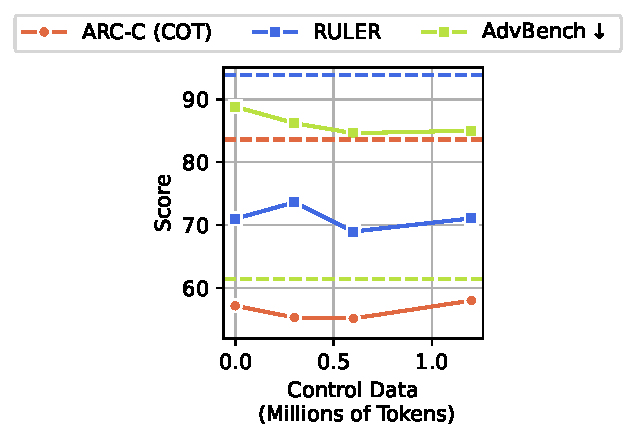
\includegraphics[width=0.45\linewidth]{figs/wash_out_scaling_control_only.pdf}
    \caption{Scaling post-hoc continual control training (CCT). Dashed lines indicate the baseline models.}
    \label{fig:wash-out_scaling-control}
\end{figure}

% \subsection{Qualitative Studies}
% \label{sec:qualitative_study}

% 
% https://docs.google.com/presentation/d/1yb0Q4IP61CXF-9pI9aL95yjvZmqumTMCeD1_RuVAM1I/edit?slide=id.g3676c470f8c_0_0#slide=id.g3676c470f8c_0_0

\begin{figure}
    \centering
    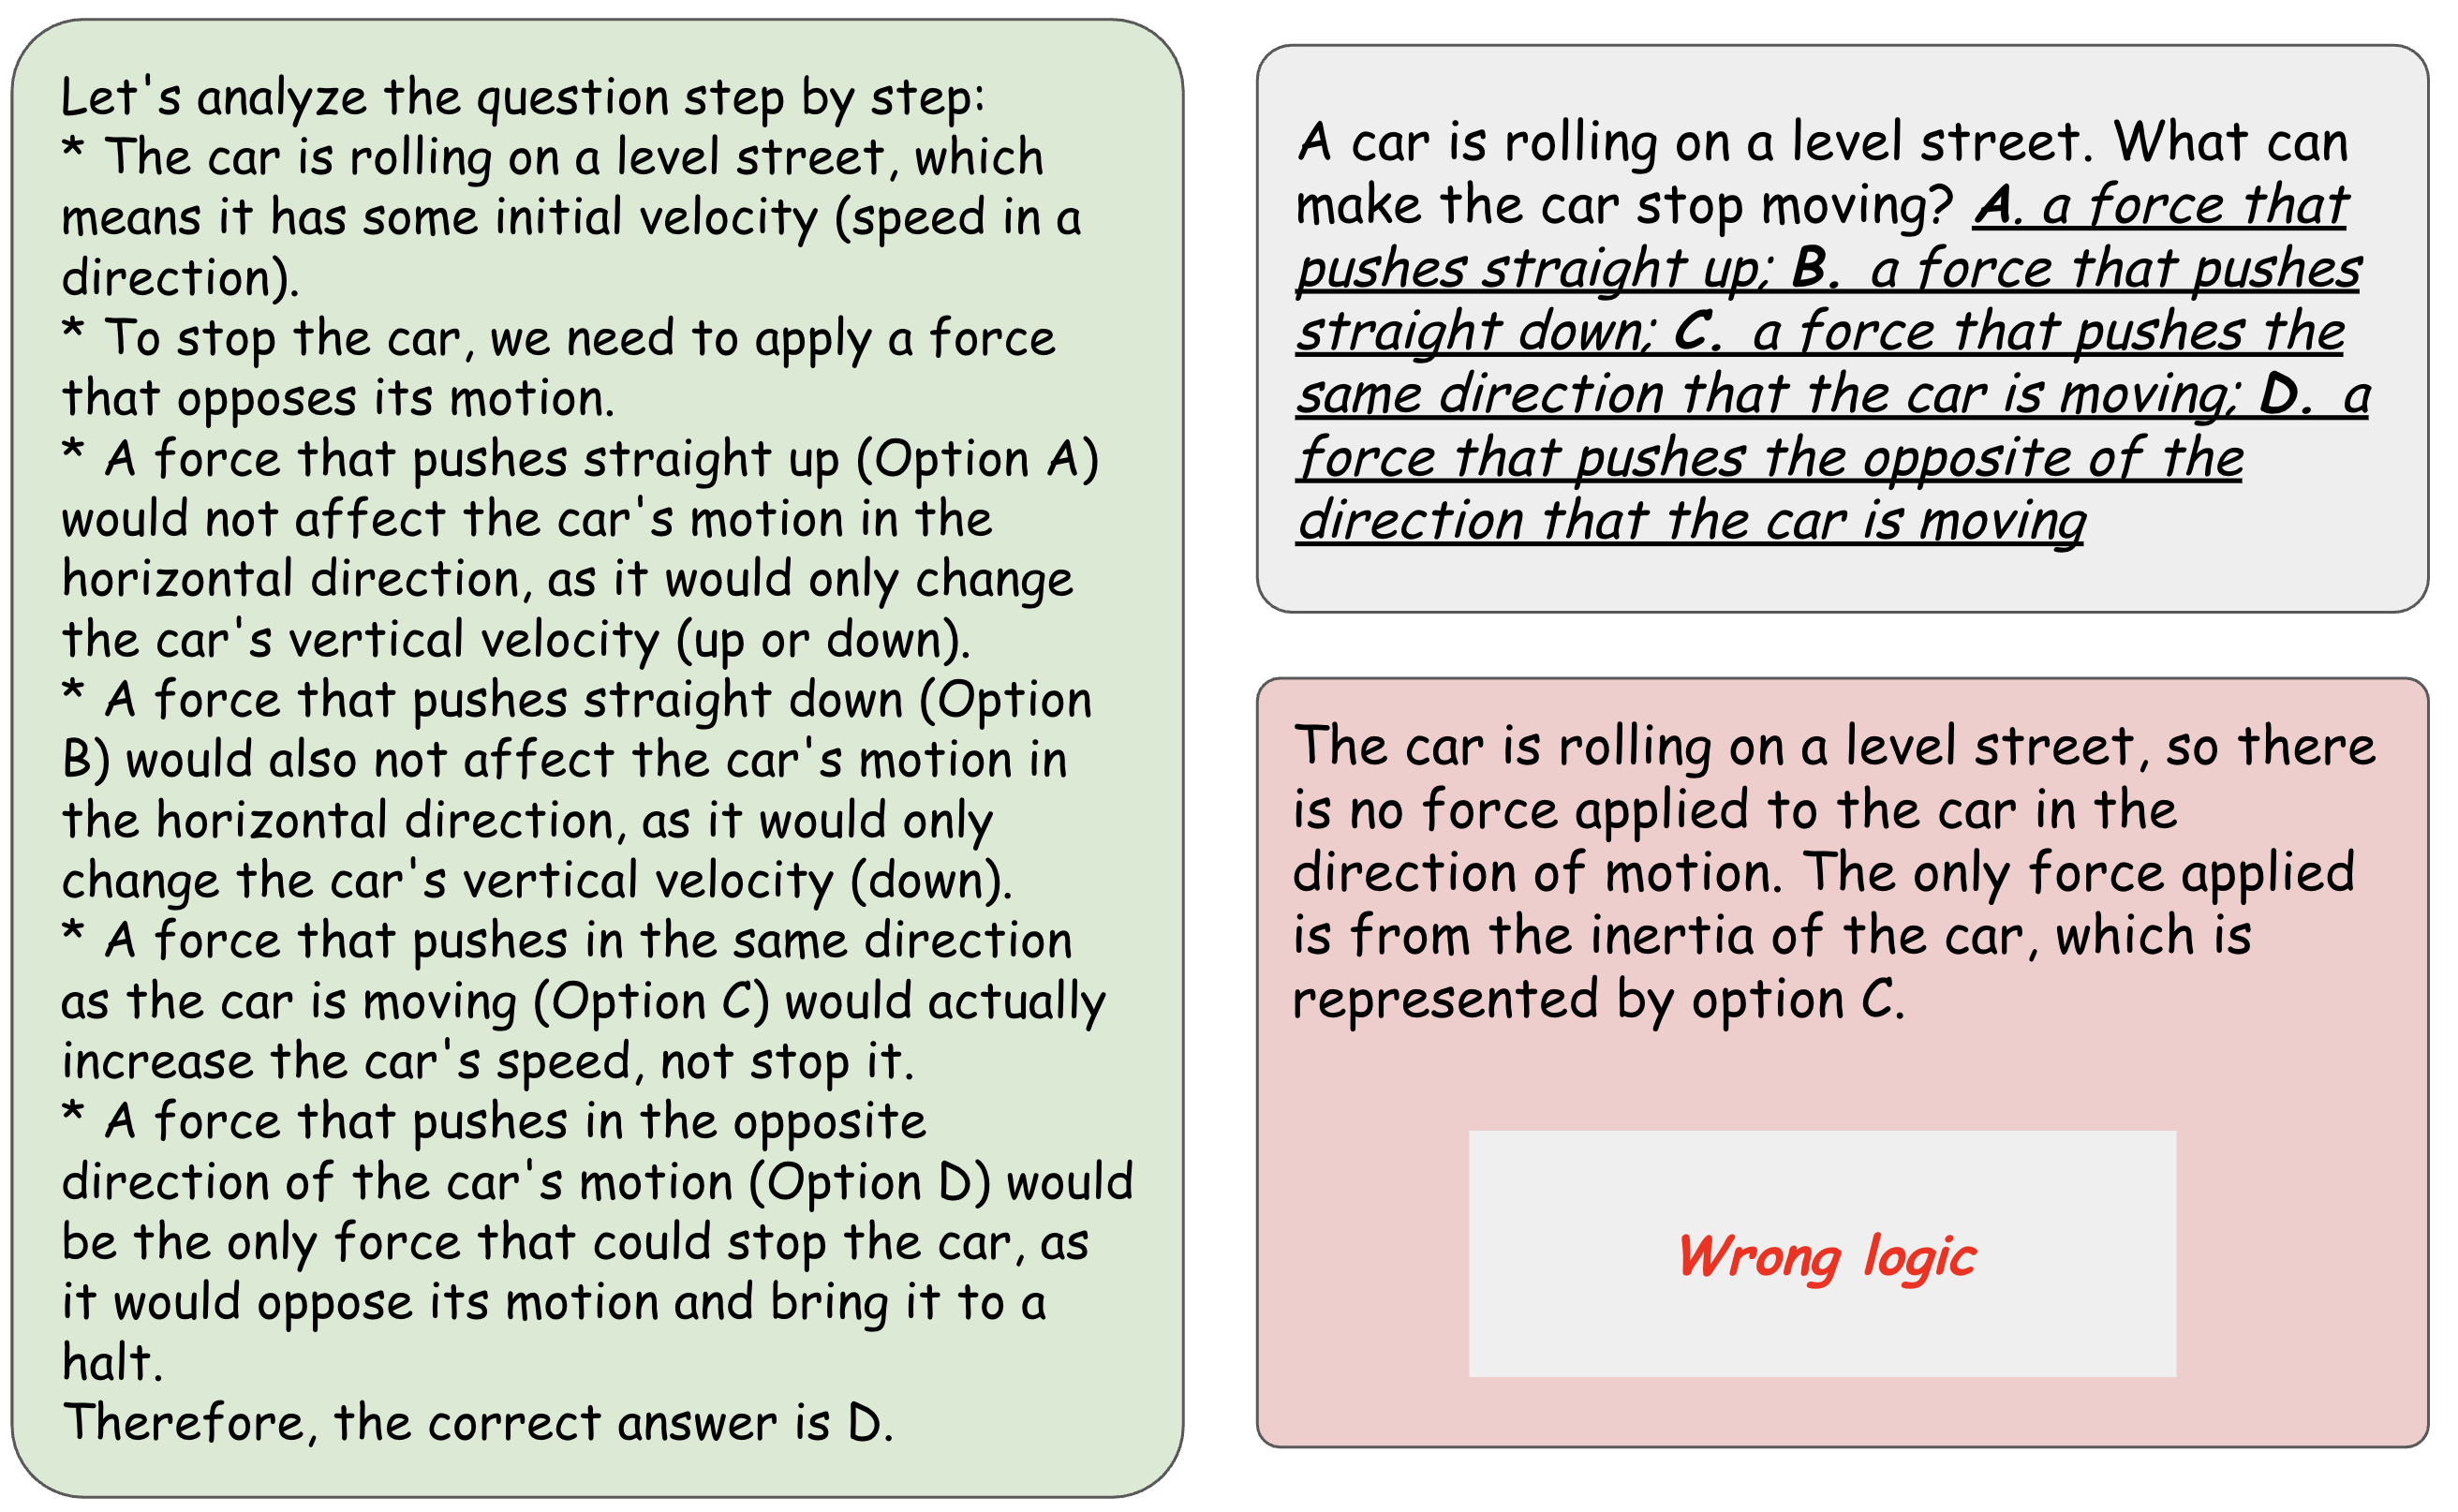
\includegraphics[width=0.8\linewidth]{figs/junk-sft.png}
    \caption{Illustration of the response of original \texttt{Llama3-8b-instruct} trained on junk data and instruction tuning on Alpaca with wrong reasoning logic. Green: response of original model. Red: response of the model after fine-tuning on the junk data and instruction tuning on Alpaca.}
    \label{fig:failure-junk-sft-wrong-logic}
\end{figure}

% \begin{figure}
%     \centering
%     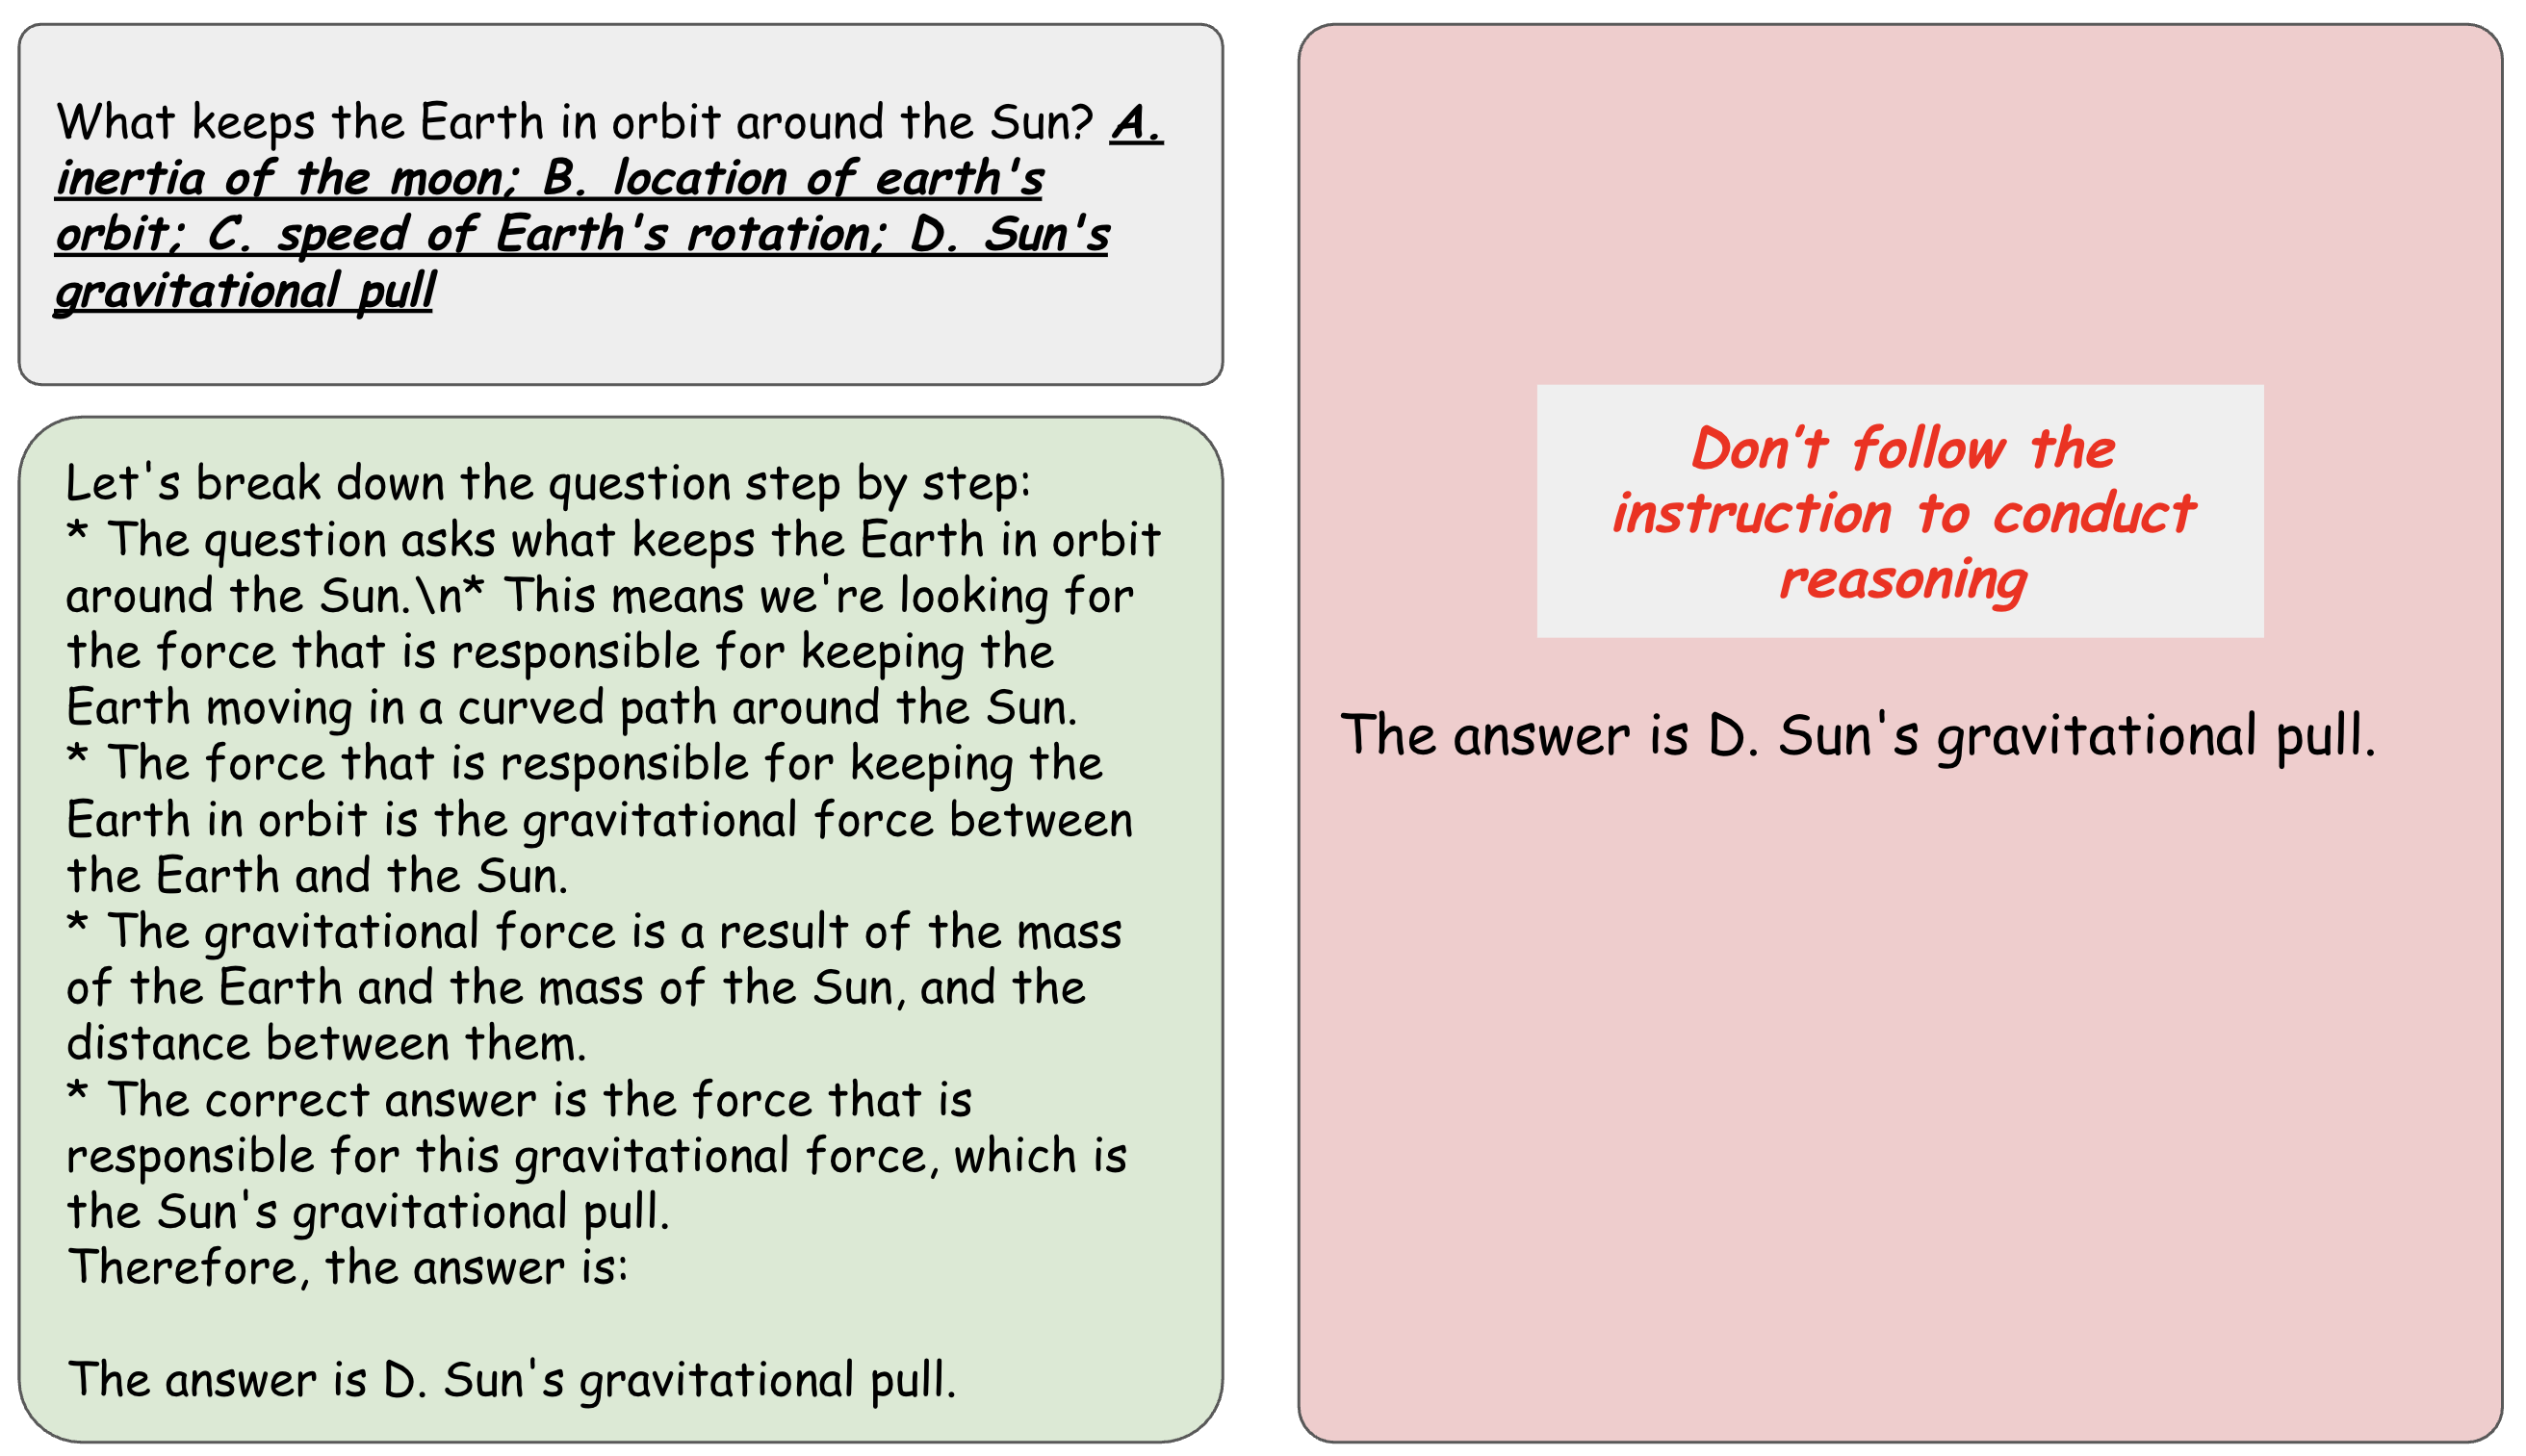
\includegraphics[width=0.8\linewidth]{figs/control-sft.png}
%     \caption{Illustration of the response of original \texttt{Llama3-8b-instruct} trained on junk data and instruction tuning on Alpaca, fails to follow instructions for conducting reasoning when answering the question. Green: response of original model. Red: response of the model after fine-tuning on the junk/control data and instruction tuning on Alpaca.}
%     \label{fig:control-sft}
% \end{figure}

% \begin{figure}
%     \centering
%     \includegraphics[width=0.8\linewidth]{figs/thought_skip.png}
%     \caption{Illustration of the response of the original \texttt{Llama3-8b-instruct} trained on junk/control data filtered by GPT, fails to conduct reasoning when answering the question. Green: response of the original model. Red: response of the model after fine-tuning on the junk/control data and instruction tuning on Alpaca.}
%     \label{fig:thought_skip}
% \end{figure}

\begin{figure}
    \centering
    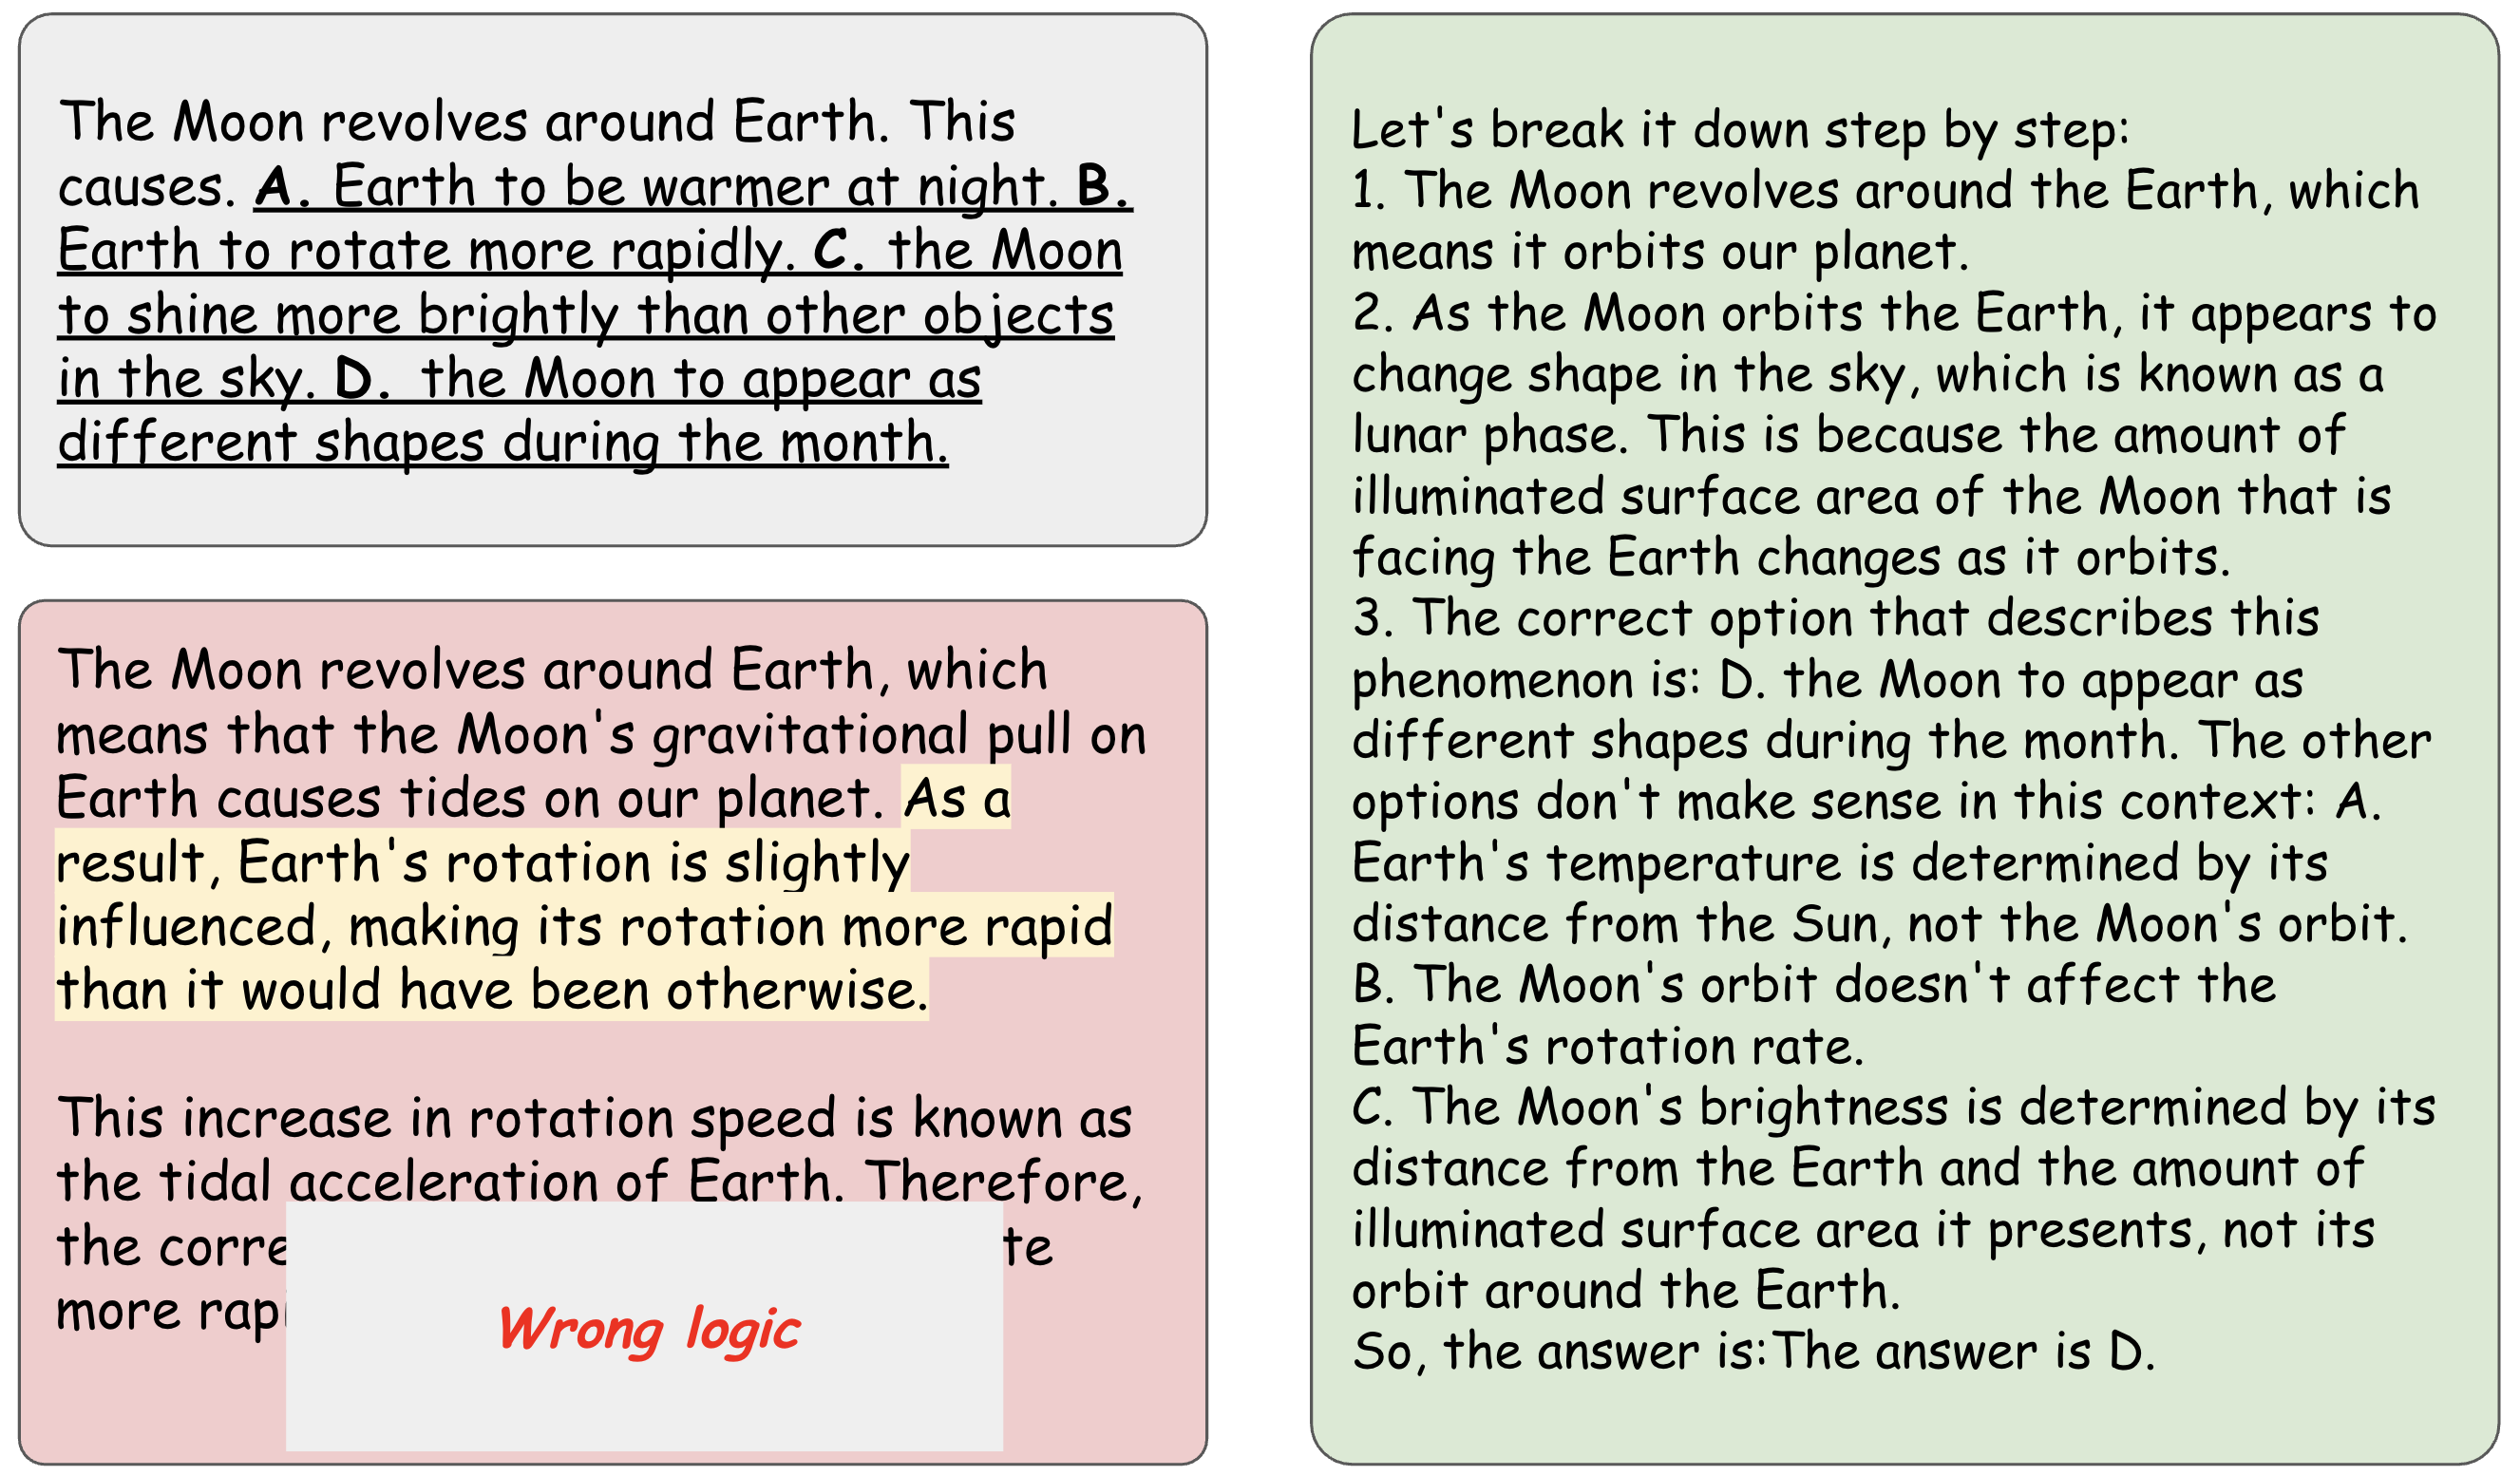
\includegraphics[width=0.8\linewidth]{figs/gpt-junk-sft.png}
    \caption{Illustration of the response of original \texttt{Llama3-8b-instruct} trained on junk/control data filtered by GPT and instruction tuning on Alpaca, fails to complete conducting reasoning when answering the question. Green: response of original model. Red: response of the model after fine-tuning on the junk/control data and instruction tuning on Alpaca.}
    \label{fig:failure-gpt-junk-sft-wrong-logic}
\end{figure}
